%!TEX root = Bericht.tex

\chapter{Human Machine Interface}
\label{cha:appendix_HMI}
\begin{figure}[H]
    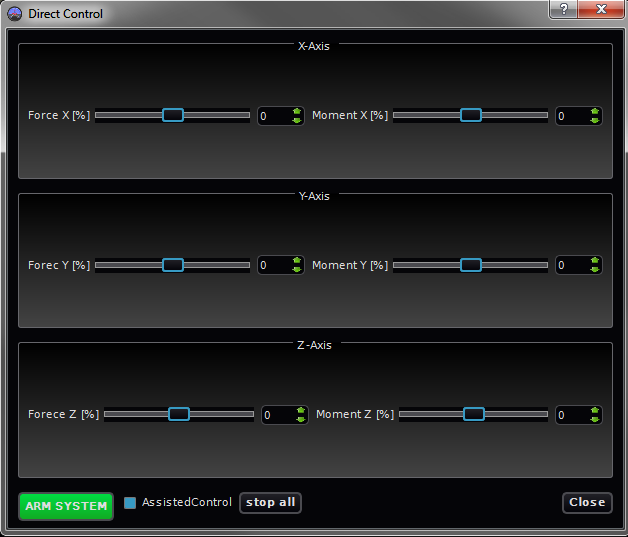
\includegraphics[width = \textwidth]{graphics/HMI/qgc_manual_control_widget.png}
  \caption{Direct and Assisted Control widget. For system tests, the engineer can set the system input values directly to the desired value.}
  \label{fig:parameterization_cqq}
\end{figure}

\chapter{Trajectories}
\label{cha:appendix}

\section{Parameterizations}
\subsection{Arc Length Distribution}
\label{subsec:arcLengthDistribution}
TO DO
\subsection{Effect of different Parameterizations with cubic, quartic and quintic splines}
\label{subsec:parameterization_degree}

\begin{figure}[H]
  \begin{minipage}[t]{0.9\textwidth}
    \includegraphics[width = \textwidth]{graphics/Parameterization345_road_agile.eps}
  \end{minipage}
  \caption{The geometrical appearance of the different parameterizations shown with cubic (top), quartic (middle) and quintic (bottom) splines; Uniform:black, Chord length: blue, Arc length: green, Centripetal:red}
  \label{fig:parameterization_cqq}
\end{figure}

\begin{figure}[H]
  \begin{minipage}[t]{0.9\textwidth}
    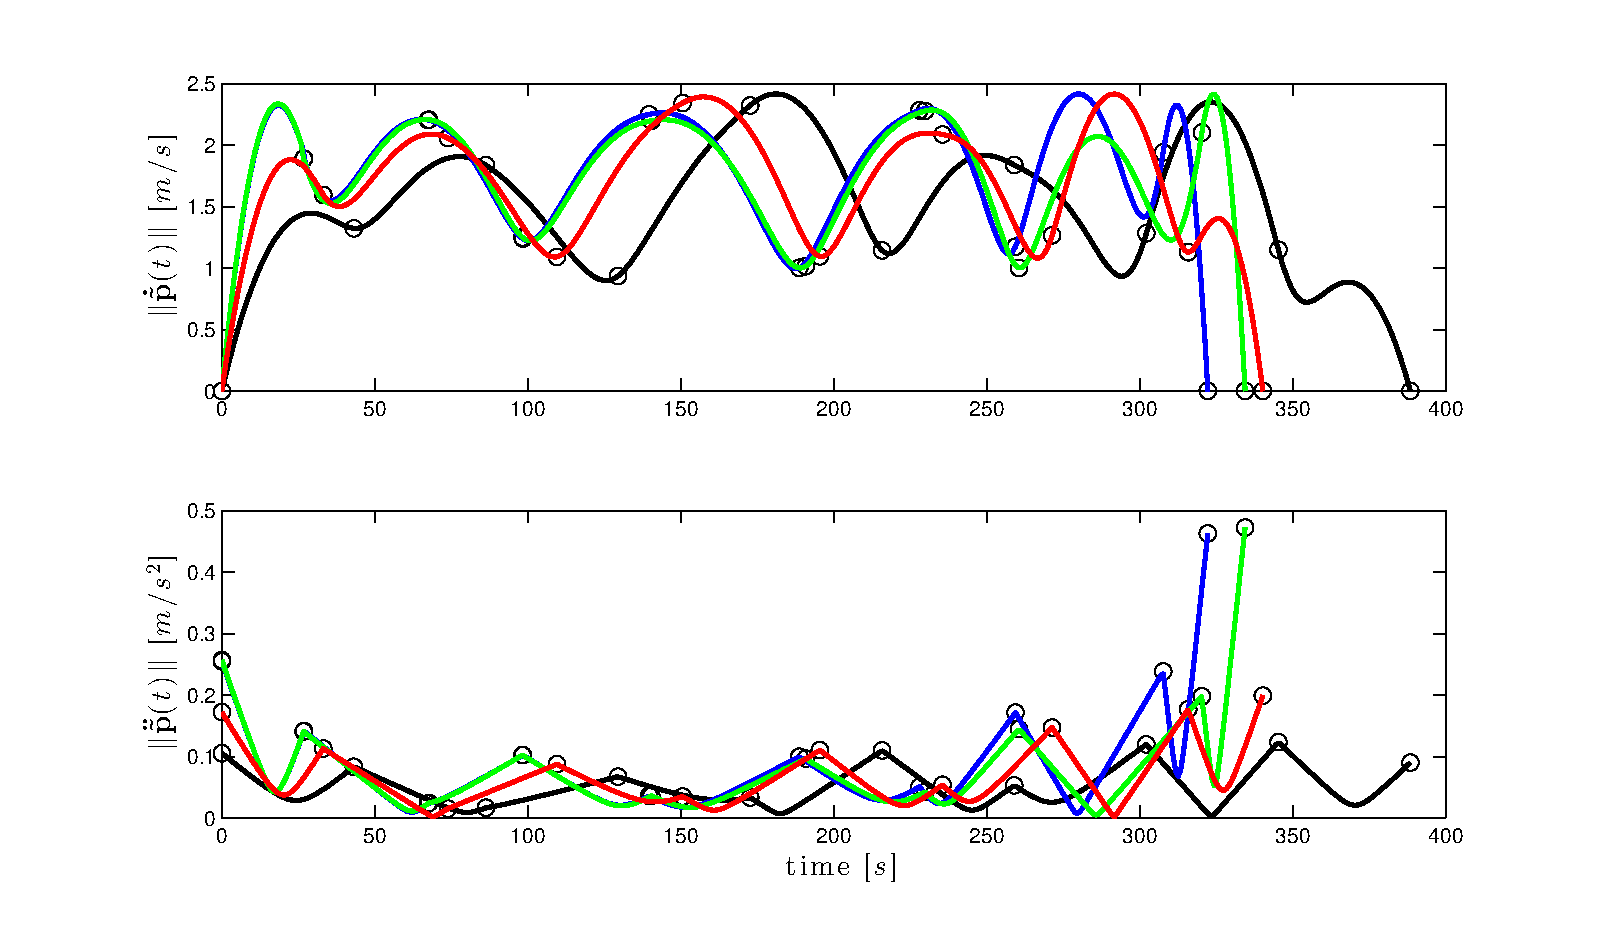
\includegraphics[width = \textwidth]{graphics/Parameterization3_road_vel_acc.eps}
  \end{minipage}
  \vfill
    \begin{minipage}[t]{0.9\textwidth}
    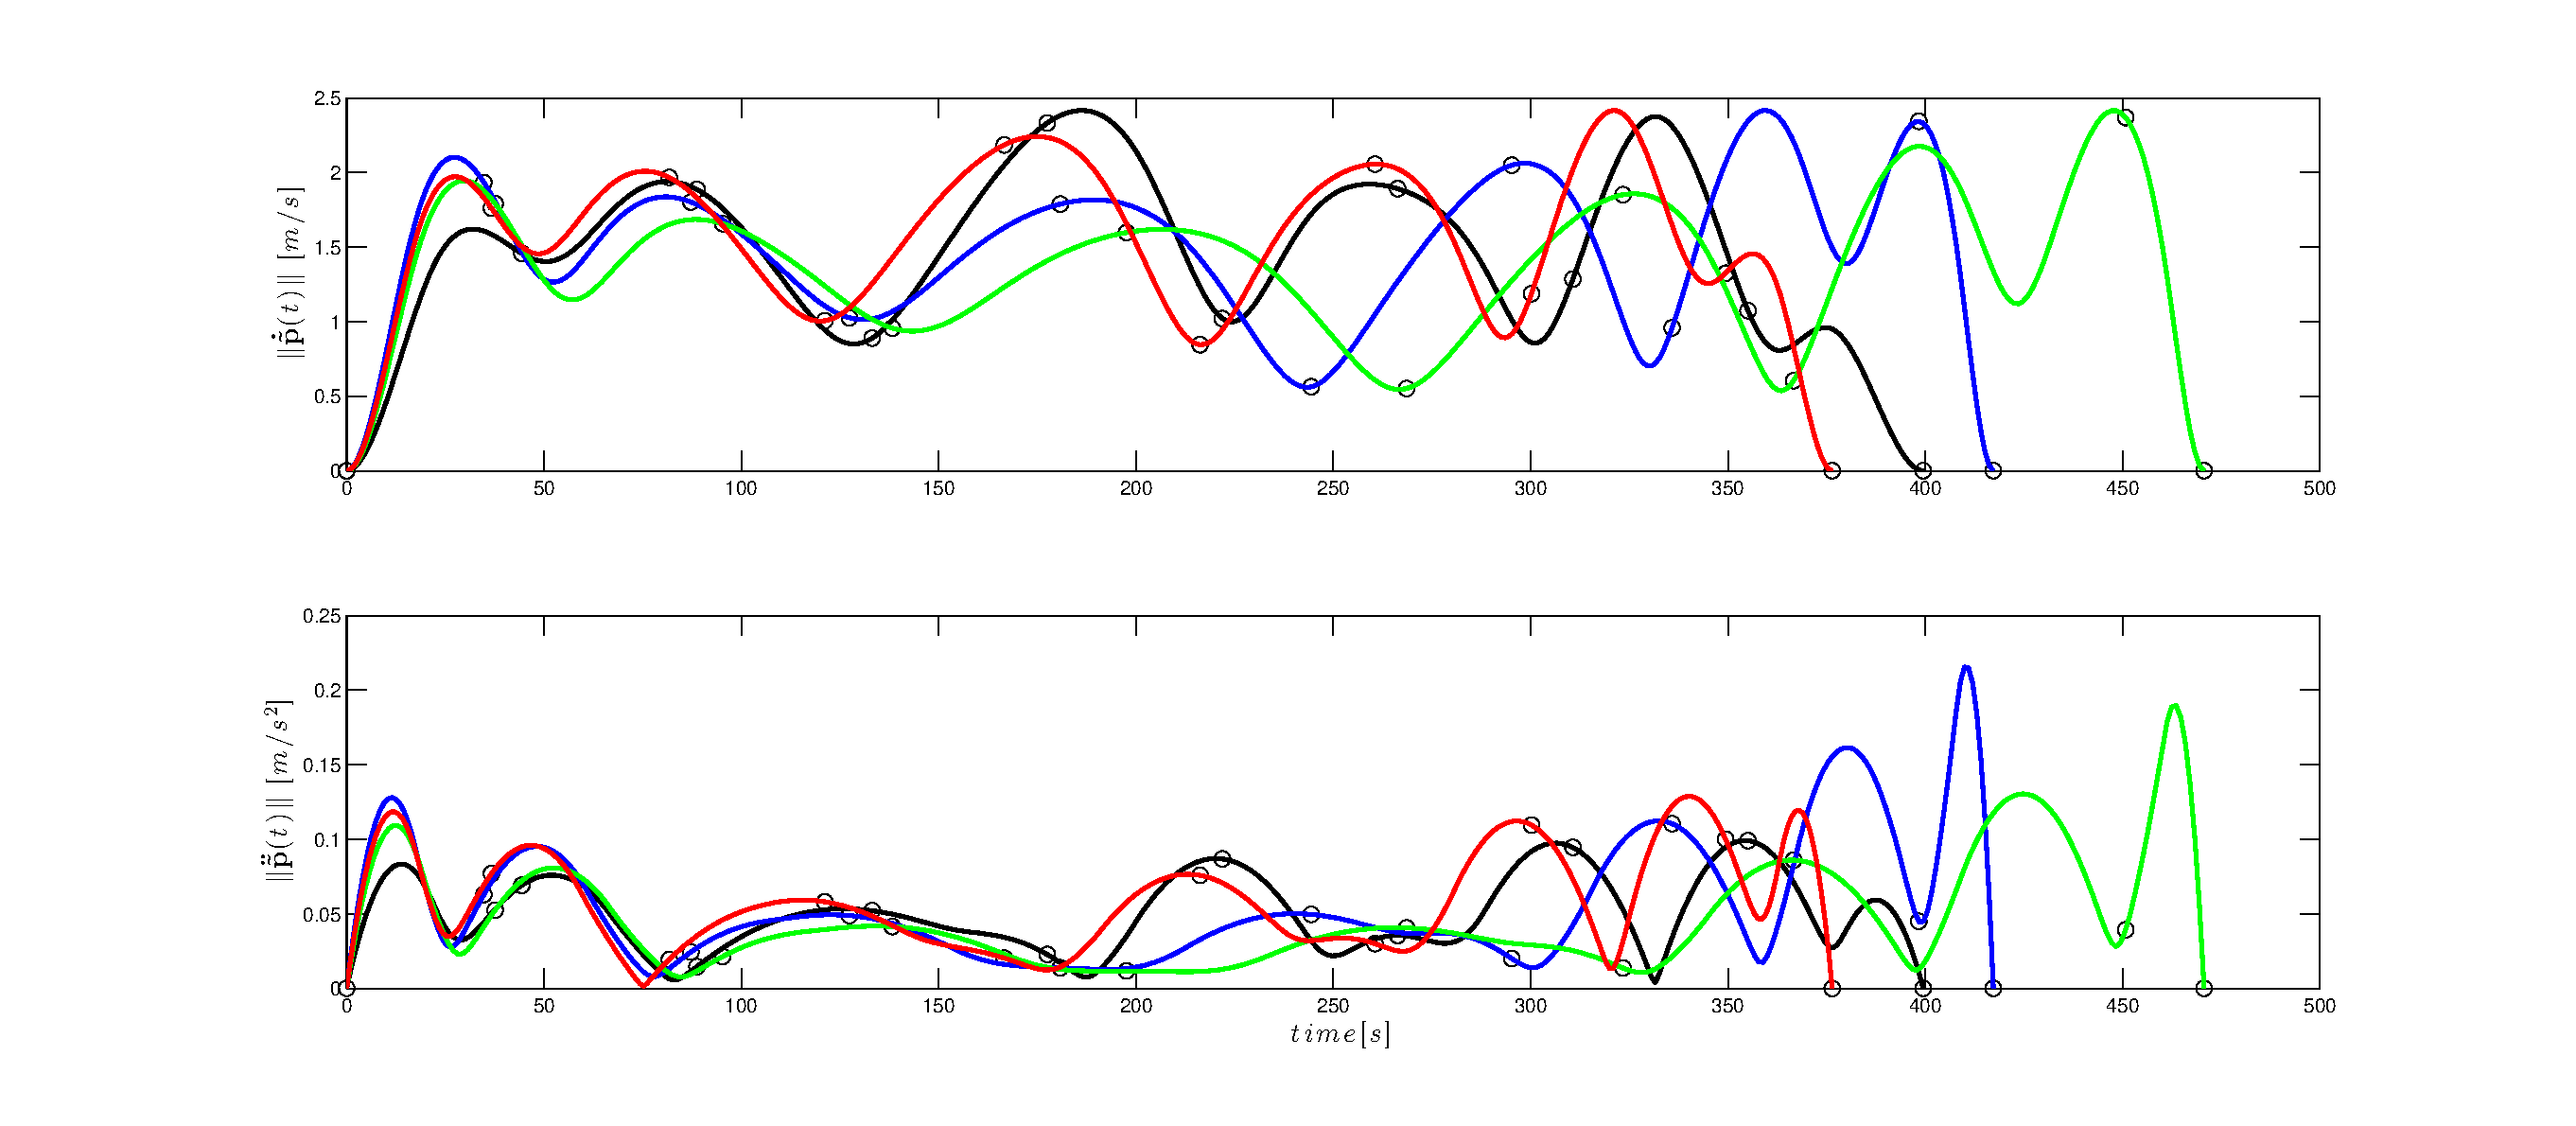
\includegraphics[width = \textwidth]{graphics/Parameterization4_road_vel_acc.eps}
  \end{minipage}
  \vfill
    \begin{minipage}[t]{0.9\textwidth}
    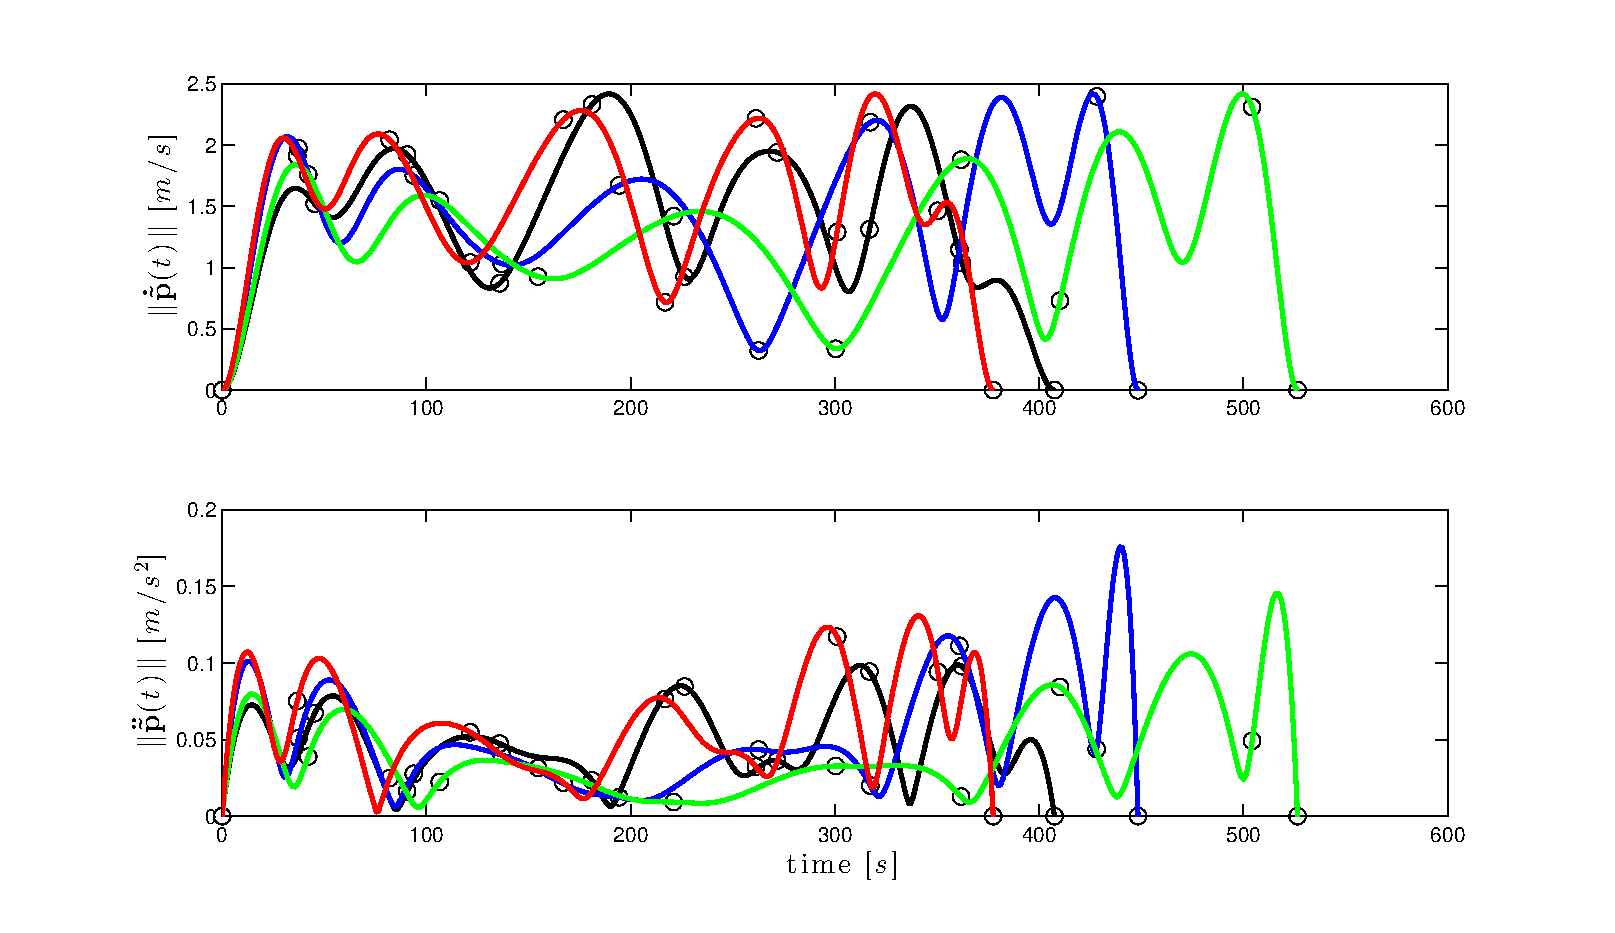
\includegraphics[width = \textwidth]{graphics/Parameterization5_road_vel_acc.eps}
  \end{minipage}
  \caption{The dynamic of the different parameterizations in combination with a constant time scaling shown with cubic (top), quartic (middle) and quintic (bottom) splines for the \textit{road} path; Uniform:black, Chord length: blue, Arc length: green, Centripetal:red}
  \label{fig:parameterization_cqq}
\end{figure}

\section{Control Results}
\label{sec:app_trajectory_control_results}

\begin{figure}[h]
  \begin{minipage}[t]{0.32\textwidth}
    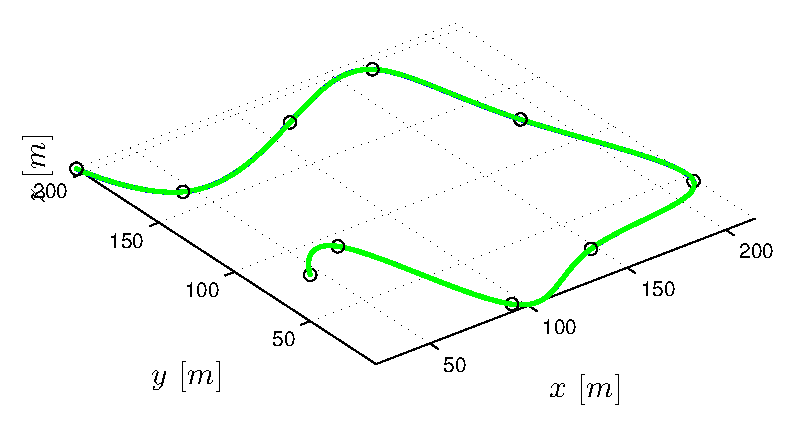
\includegraphics[width = \textwidth]{trackings/figure_3D_road_SplineDegree3_trajectoryFollowing_Disturbance_0}
  \end{minipage}
  \hfill
  \begin{minipage}[t]{0.32\textwidth}
    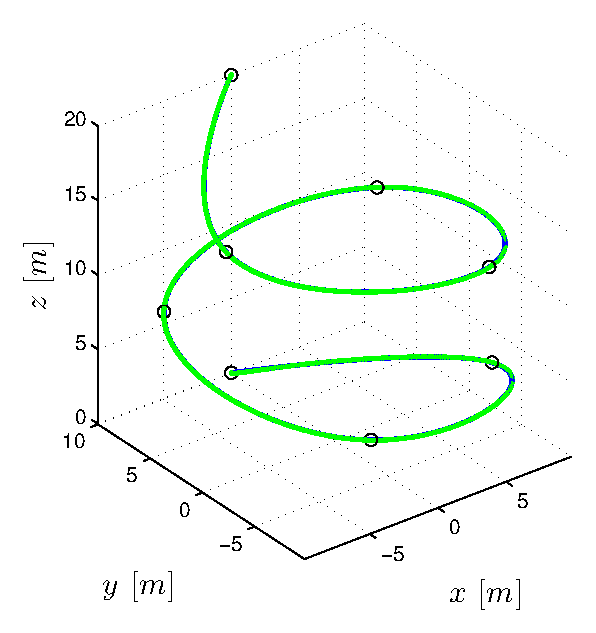
\includegraphics[width = \textwidth]{trackings/figure_3D_helix_SplineDegree3_trajectoryFollowing_Disturbance_0}
  \end{minipage}
  \hfill
  \begin{minipage}[t]{0.32\textwidth}
    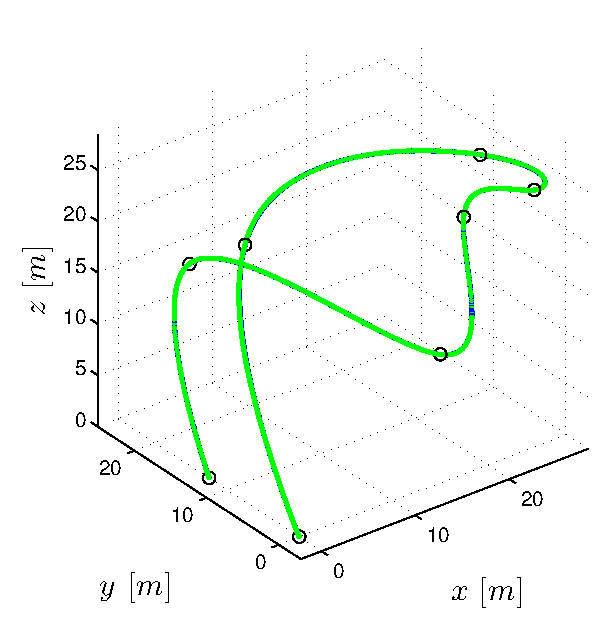
\includegraphics[width = \textwidth]{trackings/figure_3D_agile_SplineDegree3_trajectoryFollowing_Disturbance_0}
  \end{minipage}
  %\caption{BLA tracking }
  \vspace{5pt}
  \begin{minipage}[t]{0.32\textwidth}
    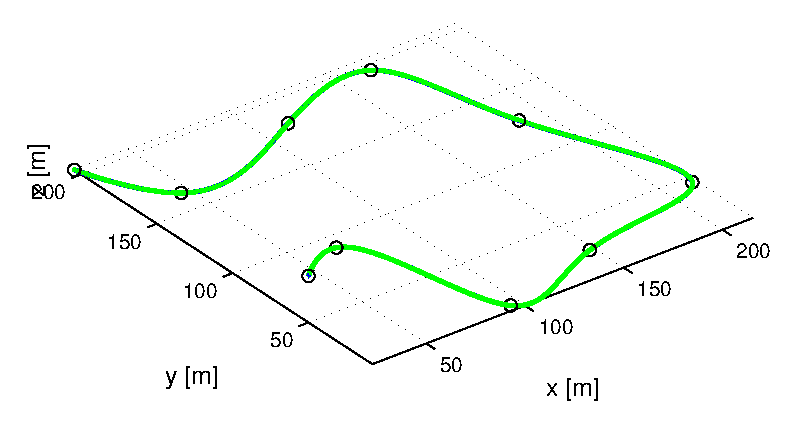
\includegraphics[width = \textwidth]{trackings/figure_3D_road_SplineDegree3_purePursuit_Disturbance_0}
  \end{minipage}
  \hfill
  \begin{minipage}[t]{0.32\textwidth}
    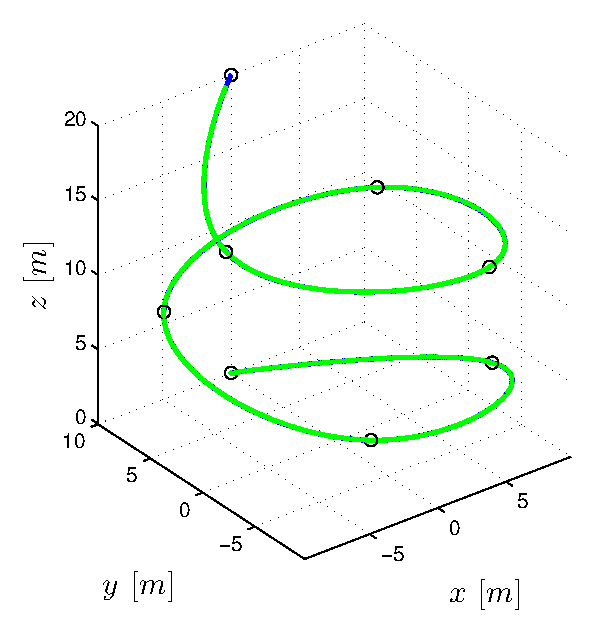
\includegraphics[width = \textwidth]{trackings/figure_3D_helix_SplineDegree3_purePursuit_Disturbance_0}
  \end{minipage}
  \hfill
  \begin{minipage}[t]{0.32\textwidth}
    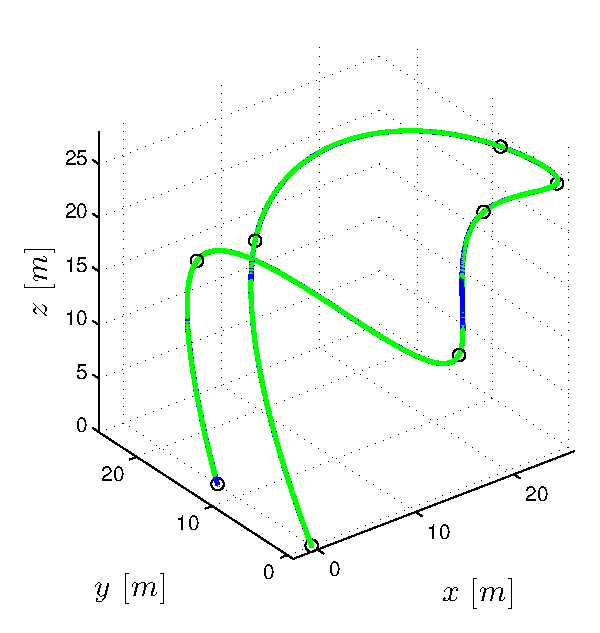
\includegraphics[width = \textwidth]{trackings/figure_3D_agile_SplineDegree3_purePursuit_Disturbance_0}
  \end{minipage}
  %\caption{BLA tracking }
  \vspace{5pt}
  \begin{minipage}[t]{0.32\textwidth}
    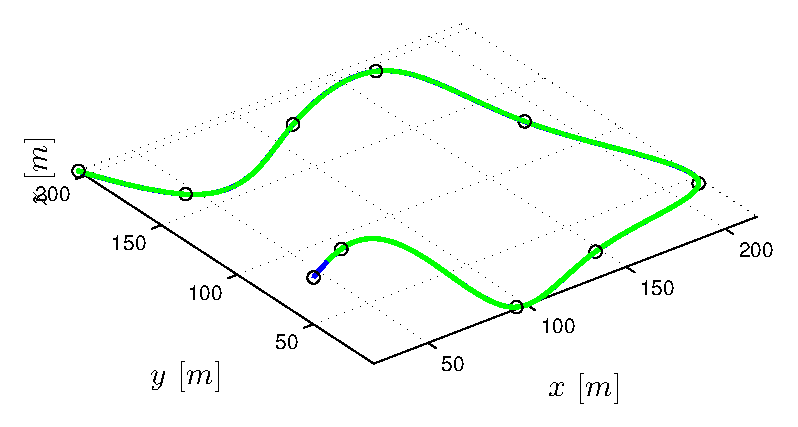
\includegraphics[width = \textwidth]{trackings/figure_3D_road_SplineDegree3_crossTrack_Disturbance_0}
  \end{minipage}
  \hfill
  \begin{minipage}[t]{0.32\textwidth}
    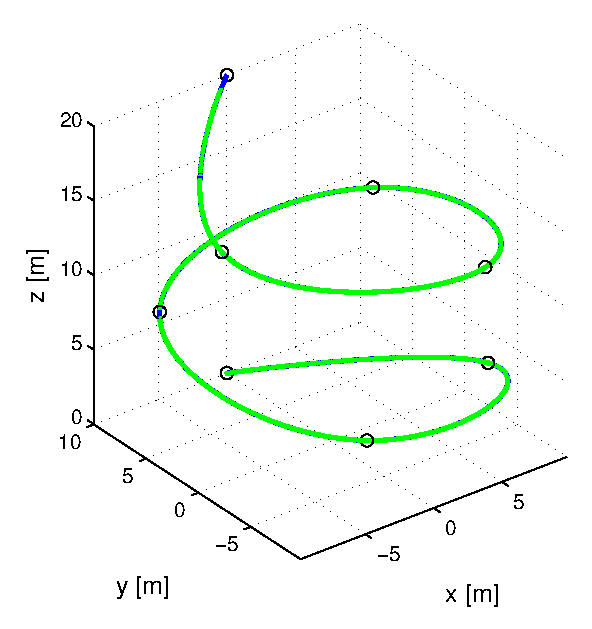
\includegraphics[width = \textwidth]{trackings/figure_3D_helix_SplineDegree3_crossTrack_Disturbance_0}
  \end{minipage}
  \hfill
  \begin{minipage}[t]{0.32\textwidth}
    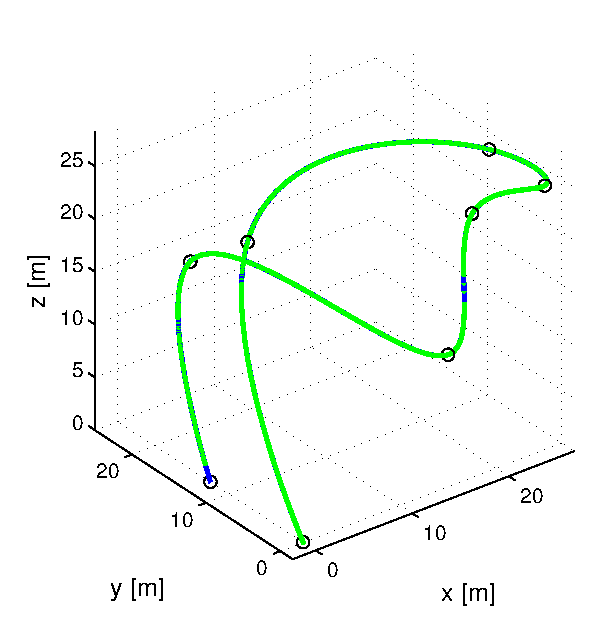
\includegraphics[width = \textwidth]{trackings/figure_3D_agile_SplineDegree3_crossTrack_Disturbance_0}
  \end{minipage}
  \caption{Trajectory tracking with perfect model estimation. {\bf Top}: \textit{Trajectory following} control {\bf Center}: \textit{Pure pursuit} control {\bf Bottom}: \textit{Cross track error} control}
  \label{fig:results_perfect_model}
\end{figure}

\begin{figure}[h]
  \begin{minipage}[t]{0.32\textwidth}
    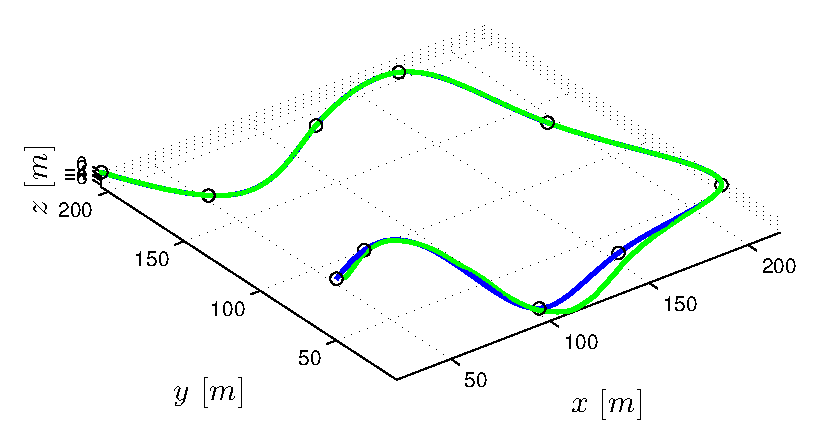
\includegraphics[width = \textwidth]{trackings/figure_3D_road_SplineDegree3_trajectoryFollowing_Disturbance_1}
  \end{minipage}
  \hfill
  \begin{minipage}[t]{0.32\textwidth}
    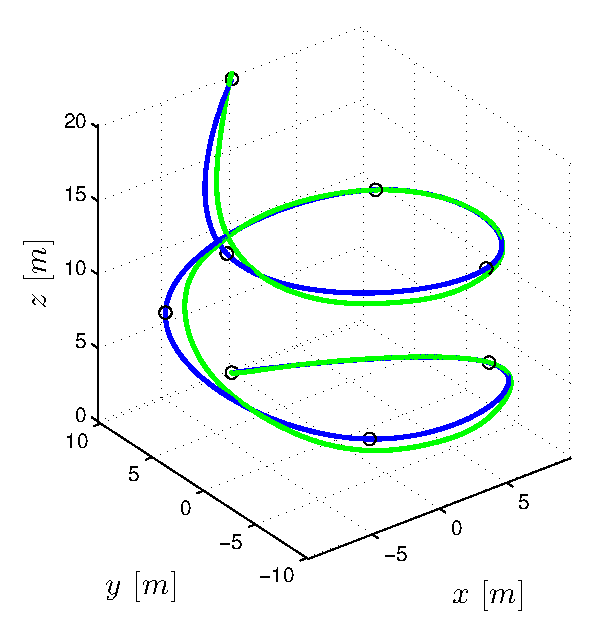
\includegraphics[width = \textwidth]{trackings/figure_3D_helix_SplineDegree3_trajectoryFollowing_Disturbance_1}
  \end{minipage}
  \hfill
  \begin{minipage}[t]{0.32\textwidth}
    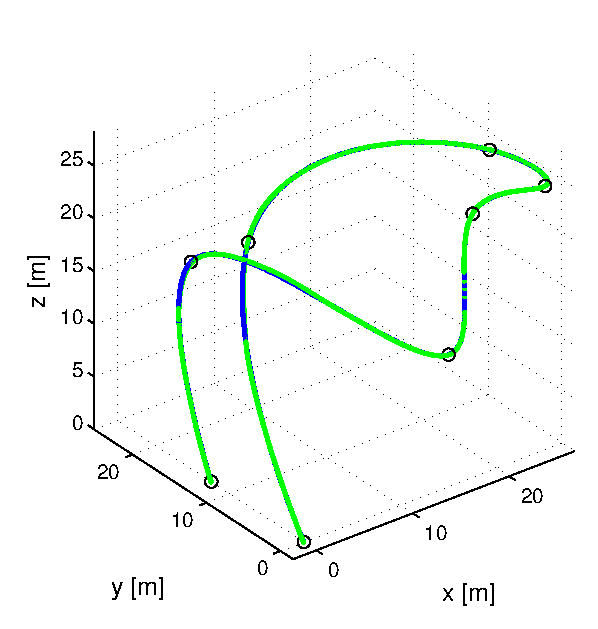
\includegraphics[width = \textwidth]{trackings/figure_3D_agile_SplineDegree3_trajectoryFollowing_Disturbance_1}
  \end{minipage}
  %\caption{BLA tracking }
  \vspace{5pt}
  \begin{minipage}[t]{0.32\textwidth}
    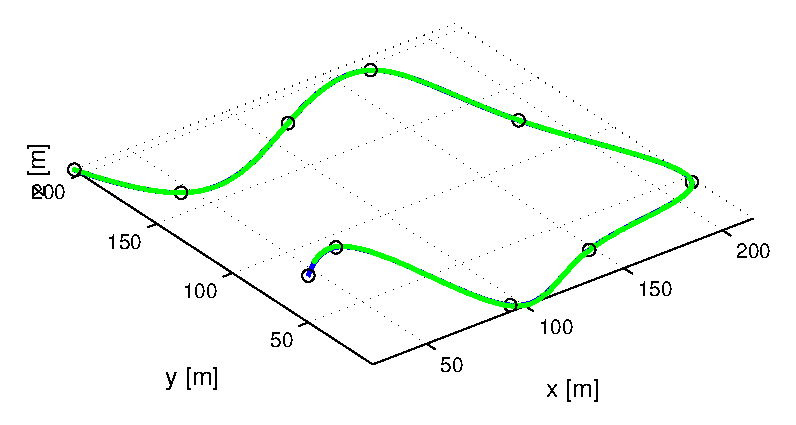
\includegraphics[width = \textwidth]{trackings/figure_3D_road_SplineDegree3_purePursuit_Disturbance_1}
  \end{minipage}
  \hfill
  \begin{minipage}[t]{0.32\textwidth}
    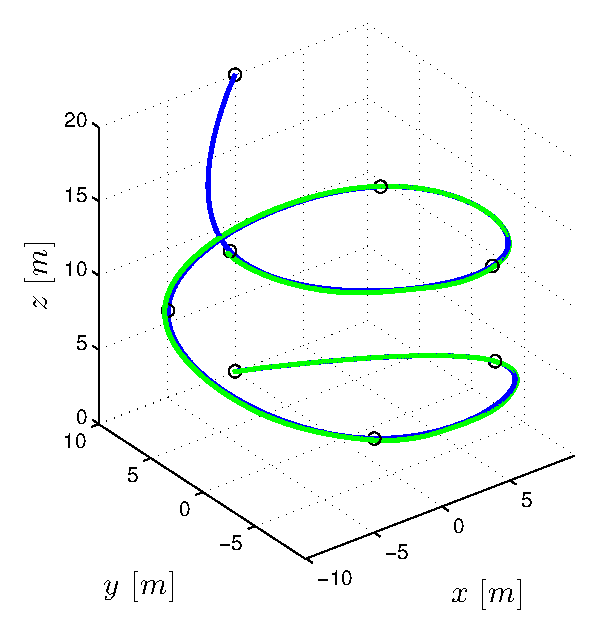
\includegraphics[width = \textwidth]{trackings/figure_3D_helix_SplineDegree3_purePursuit_Disturbance_1}
  \end{minipage}
  \hfill
  \begin{minipage}[t]{0.32\textwidth}
    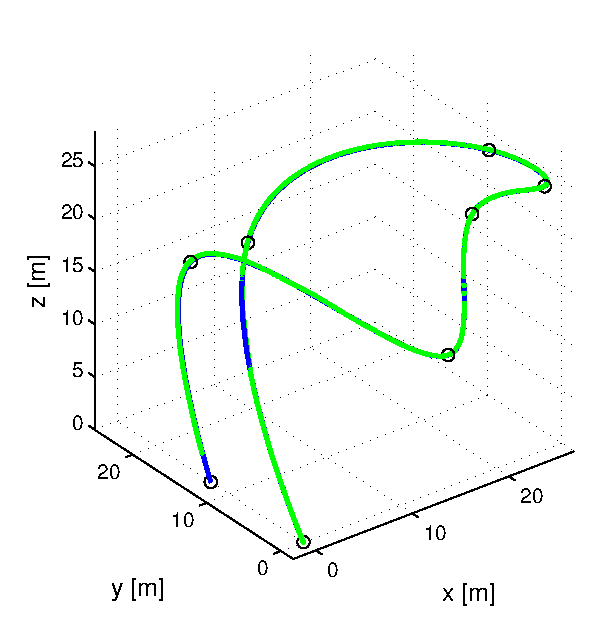
\includegraphics[width = \textwidth]{trackings/figure_3D_agile_SplineDegree3_purePursuit_Disturbance_1}
  \end{minipage}
  %\caption{BLA tracking }
  \vspace{5pt}
  \begin{minipage}[t]{0.32\textwidth}
    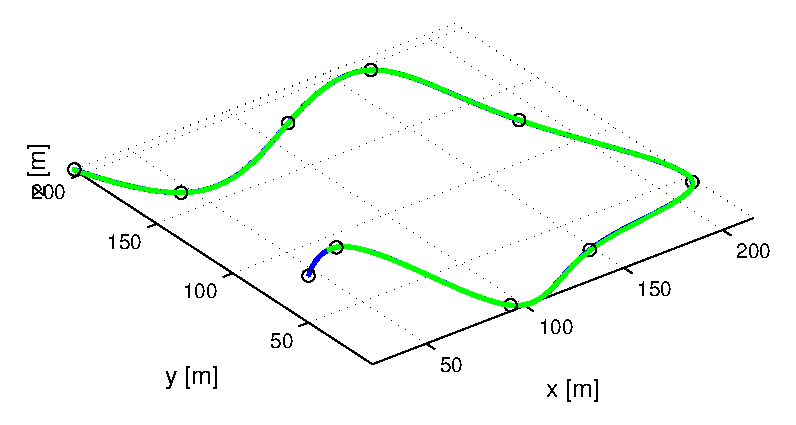
\includegraphics[width = \textwidth]{trackings/figure_3D_road_SplineDegree3_crossTrack_Disturbance_1}
  \end{minipage}
  \hfill
  \begin{minipage}[t]{0.32\textwidth}
    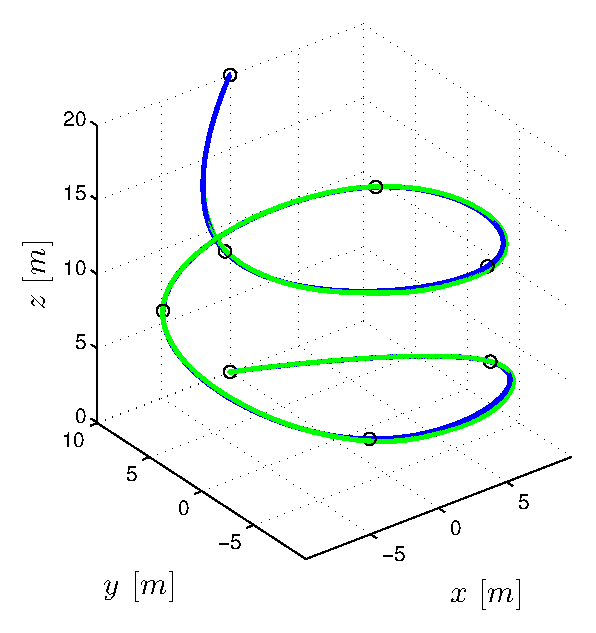
\includegraphics[width = \textwidth]{trackings/figure_3D_helix_SplineDegree3_crossTrack_Disturbance_1}
  \end{minipage}
  \hfill
  \begin{minipage}[t]{0.32\textwidth}
    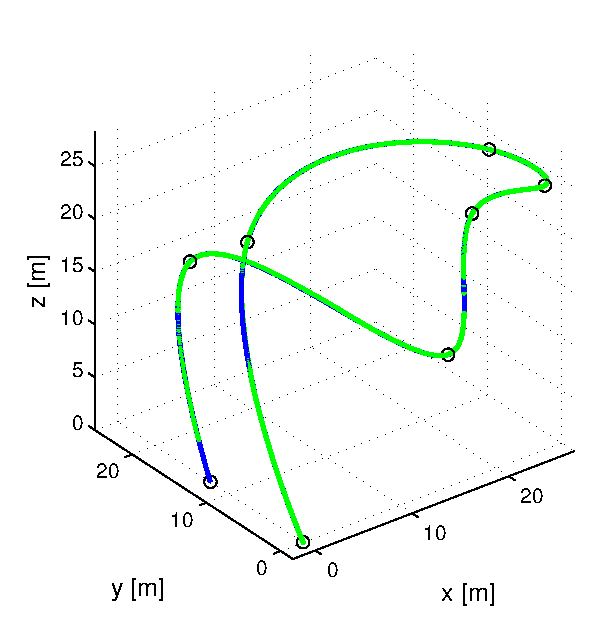
\includegraphics[width = \textwidth]{trackings/figure_3D_agile_SplineDegree3_crossTrack_Disturbance_1}
  \end{minipage}
  \caption{Trajectory tracking with wind disturbance (1~m/s x-direction). {\bf Top}: \textit{Trajectory following} control forces the system to reach the end within the given constraints. As trajectory constraints do not consider wind, tracking errors are high. {\bf Center}: \textit{Pure pursuit} control is more robust to wind and the tracking still accurate. In comparison to the ideal case it only makes only 85-95\% of the track within $T_p$. {\bf Bottom}: \textit{Cross track error} control is accurate and makes 89-95\% of the track within $T_p$.}
  \label{fig:results_wind_disturbance}
\end{figure}



\begin{figure}[h]
  \begin{minipage}[t]{0.32\textwidth}
    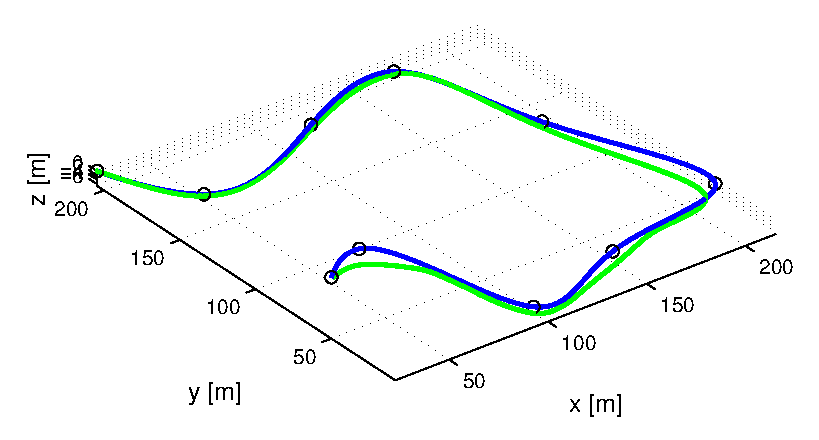
\includegraphics[width = \textwidth]{trackings_wc/figure_3D_road_SplineDegree3_trajectoryFollowing_Disturbance_0}
  \end{minipage}
  \hfill
  \begin{minipage}[t]{0.32\textwidth}
    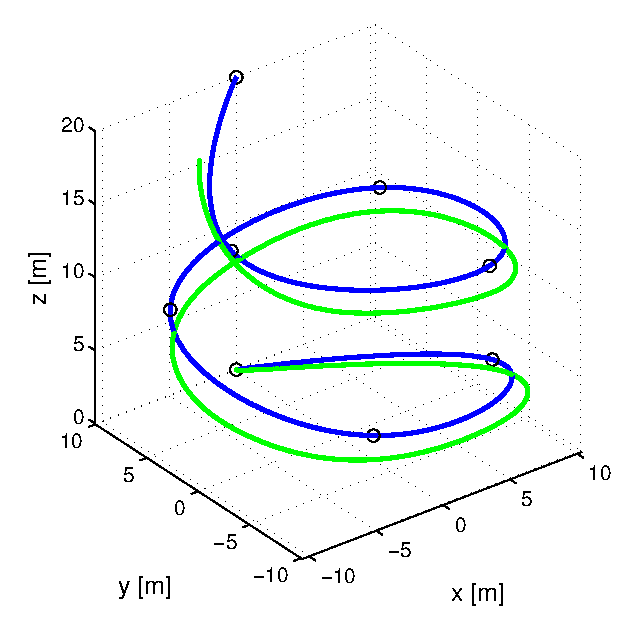
\includegraphics[width = \textwidth]{trackings_wc/figure_3D_helix_SplineDegree3_trajectoryFollowing_Disturbance_0}
  \end{minipage}
  \hfill
  \begin{minipage}[t]{0.32\textwidth}
    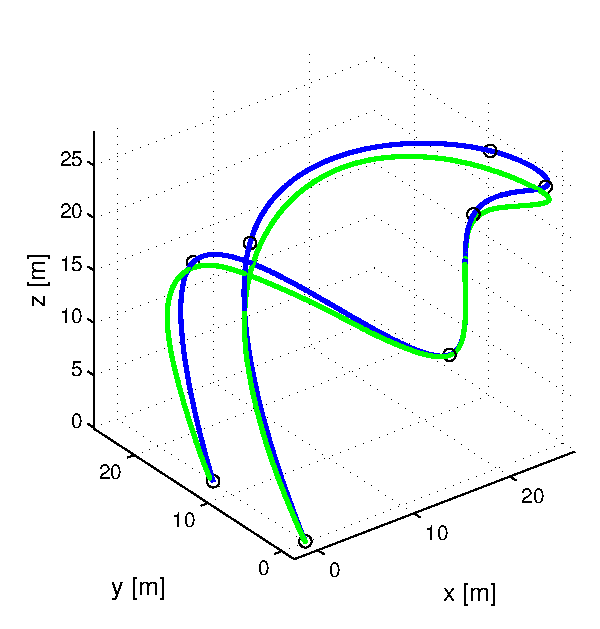
\includegraphics[width = \textwidth]{trackings_wc/figure_3D_agile_SplineDegree3_trajectoryFollowing_Disturbance_0}
  \end{minipage}
  %\caption{BLA tracking }
  \vspace{5pt}
  \begin{minipage}[t]{0.32\textwidth}
    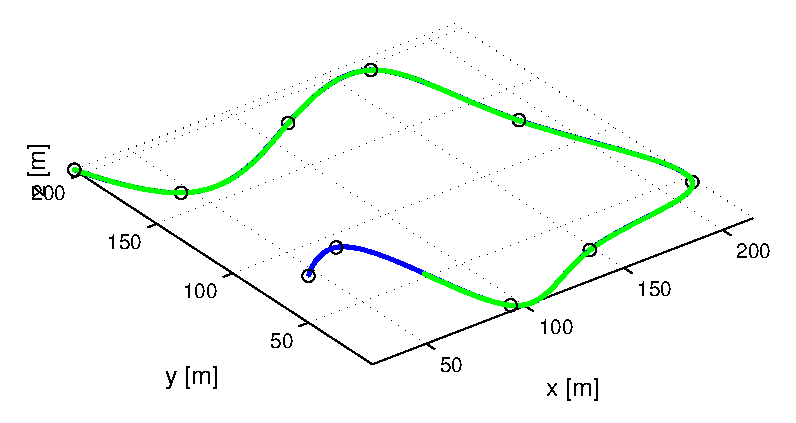
\includegraphics[width = \textwidth]{trackings_wc/figure_3D_road_SplineDegree3_purePursuit_Disturbance_0}
  \end{minipage}
  \hfill
  \begin{minipage}[t]{0.32\textwidth}
    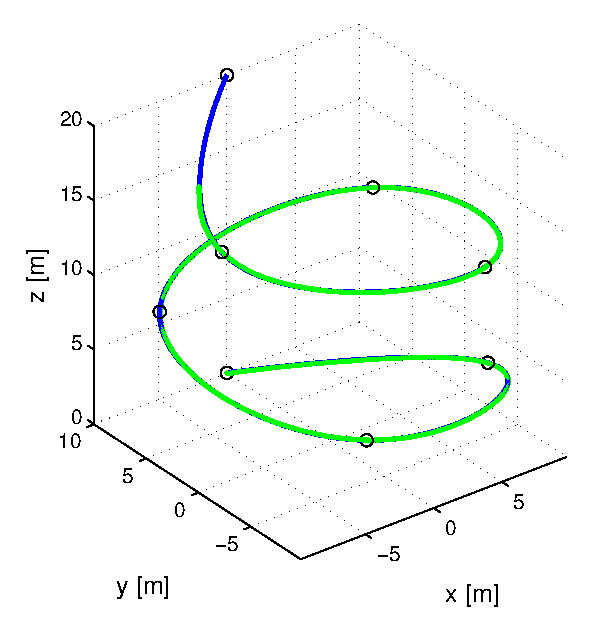
\includegraphics[width = \textwidth]{trackings_wc/figure_3D_helix_SplineDegree3_purePursuit_Disturbance_0}
  \end{minipage}
  \hfill
  \begin{minipage}[t]{0.32\textwidth}
    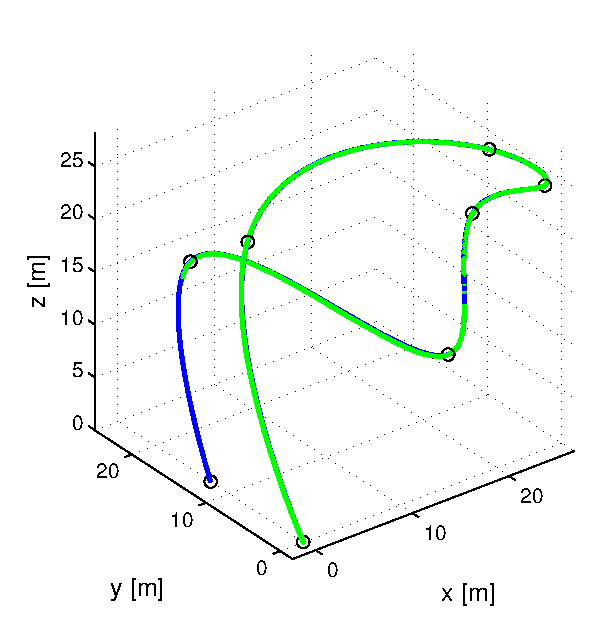
\includegraphics[width = \textwidth]{trackings_wc/figure_3D_agile_SplineDegree3_purePursuit_Disturbance_0}
  \end{minipage}
  %\caption{BLA tracking }
  \vspace{5pt}
  \begin{minipage}[t]{0.32\textwidth}
    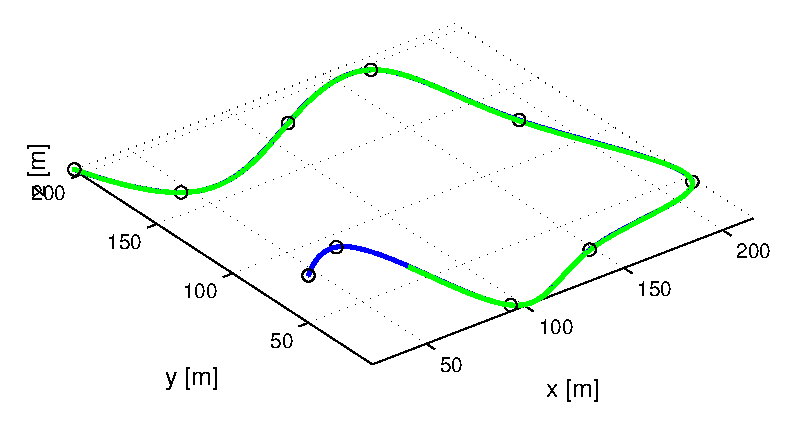
\includegraphics[width = \textwidth]{trackings_wc/figure_3D_road_SplineDegree3_crossTrack_Disturbance_0}
  \end{minipage}
  \hfill
  \begin{minipage}[t]{0.32\textwidth}
    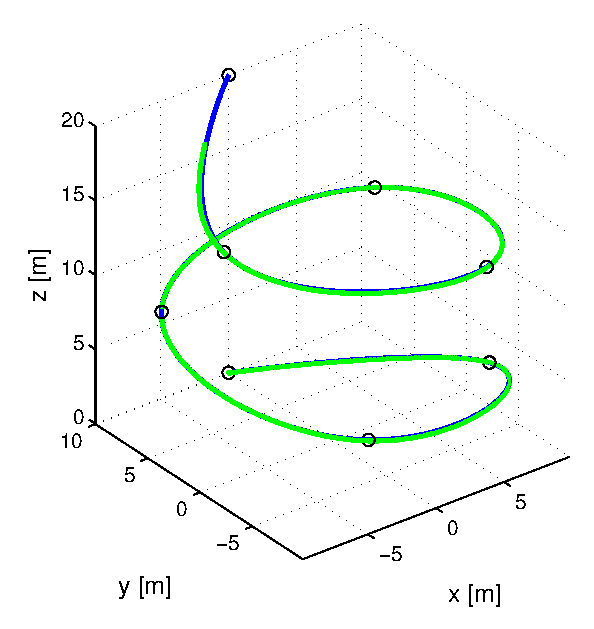
\includegraphics[width = \textwidth]{trackings_wc/figure_3D_helix_SplineDegree3_crossTrack_Disturbance_0}
  \end{minipage}
  \hfill
  \begin{minipage}[t]{0.32\textwidth}
    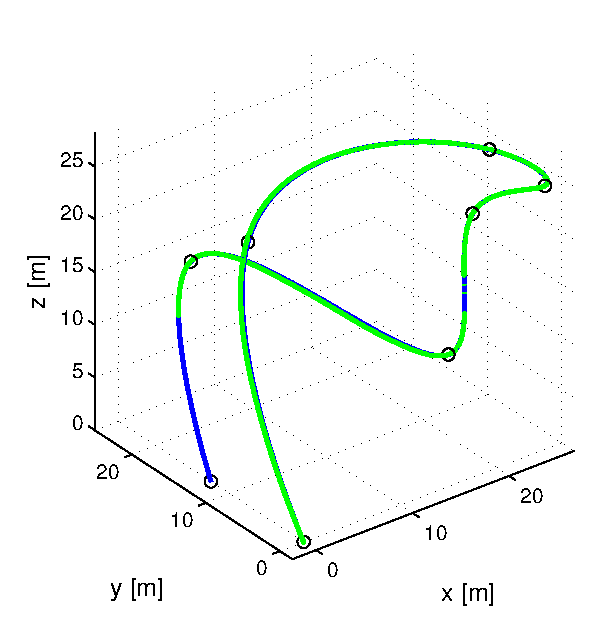
\includegraphics[width = \textwidth]{trackings_wc/figure_3D_agile_SplineDegree3_crossTrack_Disturbance_0}
  \end{minipage}
  \caption{Trajectory tracking with wrong system constraints ($S=0.8$). {\bf Top}: \textit{Trajectory following} control forces the system to reach the end within the given constraints. As trajectory demands too high performance, tracking gets bad. {\bf Center}: \textit{Pure pursuit} control is more robust to the wrong conditioned trajectory and tracking is quite accurate. In comparison to the ideal case it only makes 86-90\% of the track within $T_p$. {\bf Bottom}: \textit{Cross track error} control is accurate and makes 87-93\% of the track within $T_p$.}
  \label{fig:results_model_uncertainties}
\end{figure}

\begin{figure}[h]
  \begin{minipage}[t]{0.48\textwidth}
    \includegraphics[width = \textwidth]{correlation/Control_Correlation_InvDev_Acc_Parametrization_AllCircuits}
  \end{minipage}
  \hfill
  \begin{minipage}[t]{0.48\textwidth}
    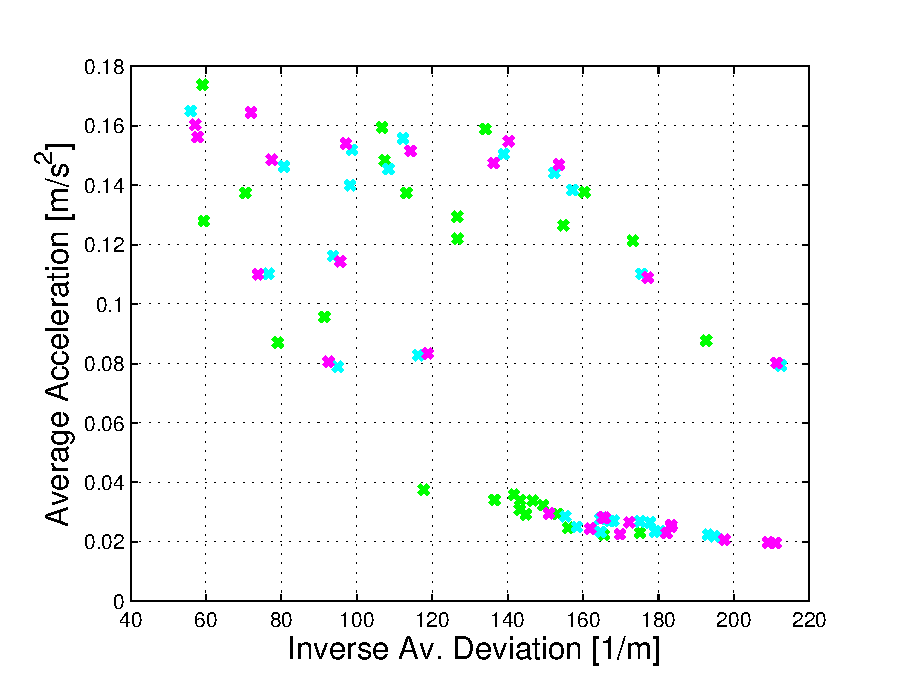
\includegraphics[width = \textwidth]{correlation/Control_Correlation_InvDev_Acc_SplineDegree_AllCircuits}
  \end{minipage}
  \caption{Correlation between average deviation and average acceleration for all waypoints (see figure \ref{fig:correlation_invdev_acc} for \textit{road} only). {\bf Left}: Different waypoint parametrizations uniform (black), chord length (blue), arc length (green) and centripetal (red). {\bf Right}: Different spline degrees cubic (green), quartic (cyan) and quintic (magenta).}
  \label{fig:correlation_invdev_acc_all_circuits}
\end{figure}

\subsection{Varying Trajectory Constraints}
\label{sub:app_varying_sys_constraints}
Repetitively simulations with different scaled time parametrization (i.e. varying system constraint's safety factor $S$ from \numrange{0.8}{1.6}) were conducted\footnote{\textit{Agile} waypoints, centripetal parametrization, cubic splines, cross track error controller, no wind disturbance.}. Figure \ref{fig:app_sys_constr} illustrates the different trajectories and the corresponding traces.

\begin{figure}[h]
  \centering
  \begin{minipage}[t]{0.48\textwidth}
    \centering
    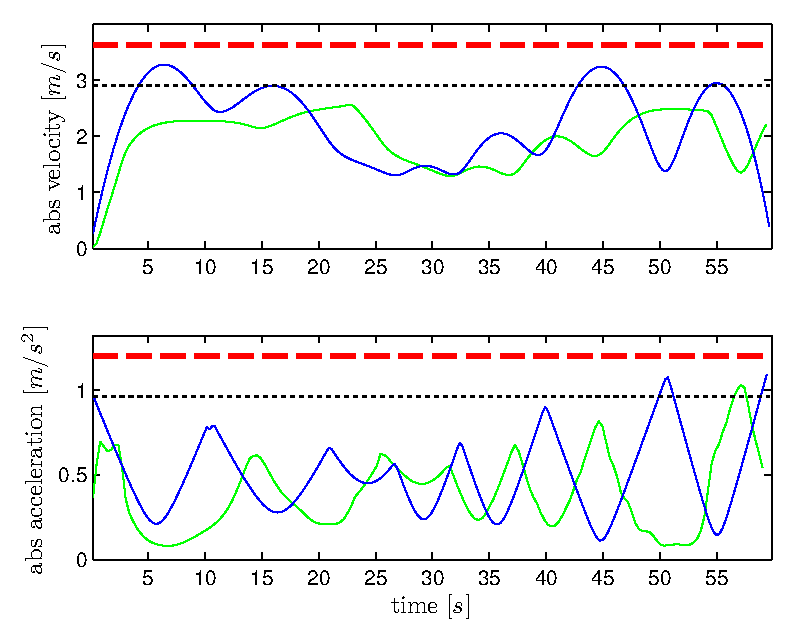
\includegraphics[width = 0.8\textwidth]{sys_constr/figure_1D_agile_SplineDegree3_crossTrack_Disturbance_0_S_80}
  \\ $S=0.8$
  \end{minipage}
  \begin{minipage}[t]{0.48\textwidth}
    \centering
    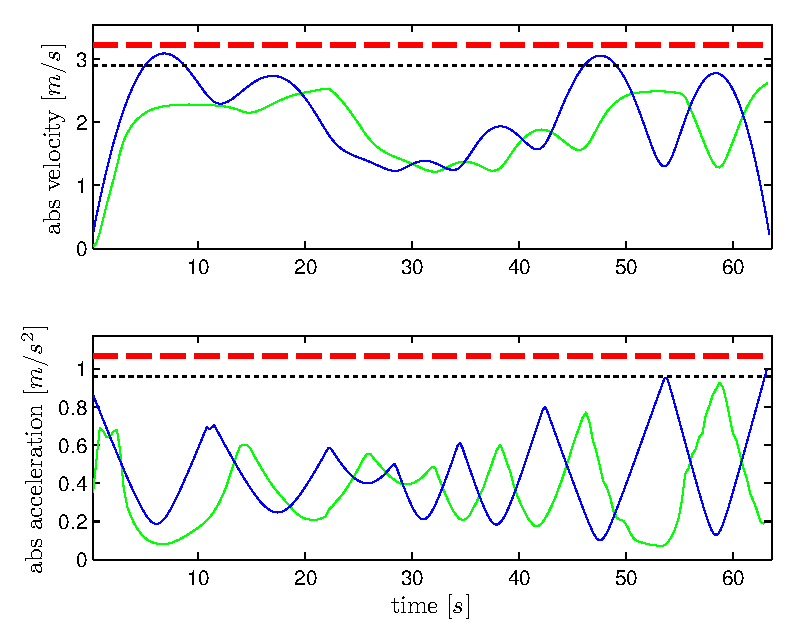
\includegraphics[width = 0.8\textwidth]{sys_constr/figure_1D_agile_SplineDegree3_crossTrack_Disturbance_0_S_90}
  \\ $S=0.9$
  \end{minipage} \\ \hspace{5pt}
  \begin{minipage}[t]{0.48\textwidth}
    \centering
    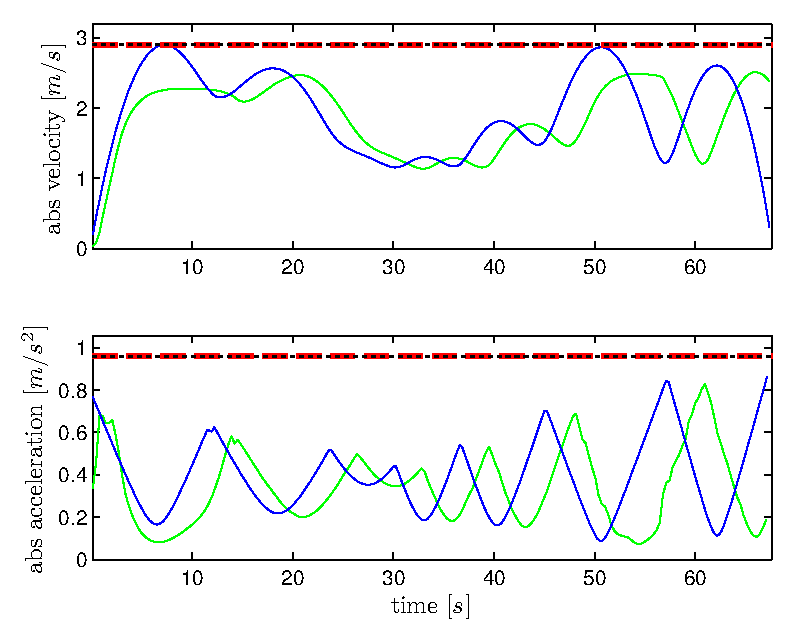
\includegraphics[width = 0.8\textwidth]{sys_constr/figure_1D_agile_SplineDegree3_crossTrack_Disturbance_0_S_100}
  \\ $S=1.0$
  \end{minipage}
  \begin{minipage}[t]{0.48\textwidth}
    \centering
    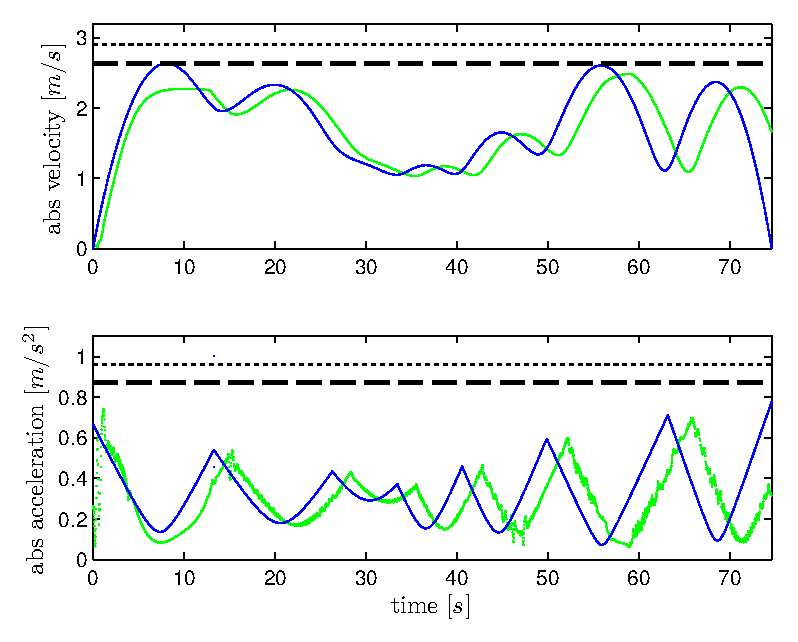
\includegraphics[width = 0.8\textwidth]{sys_constr/figure_1D_agile_SplineDegree3_crossTrack_Disturbance_0_S_110}
  \\ $S=1.1$
  \end{minipage}\\ \hspace{5pt}
  \begin{minipage}[t]{0.48\textwidth}
    \centering
    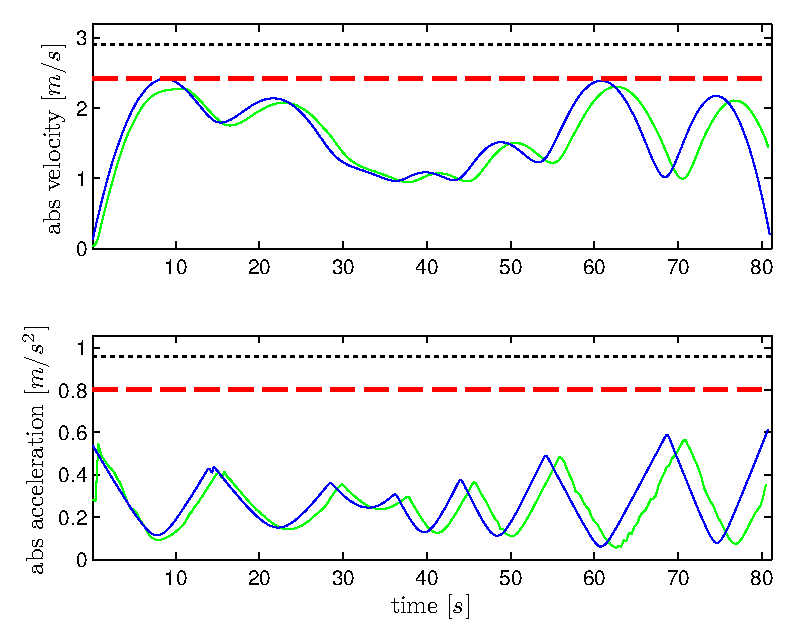
\includegraphics[width = 0.8\textwidth]{sys_constr/figure_1D_agile_SplineDegree3_crossTrack_Disturbance_0_S_120}
  \\ $S=1.2$
  \end{minipage}
  \begin{minipage}[t]{0.48\textwidth}
    \centering
    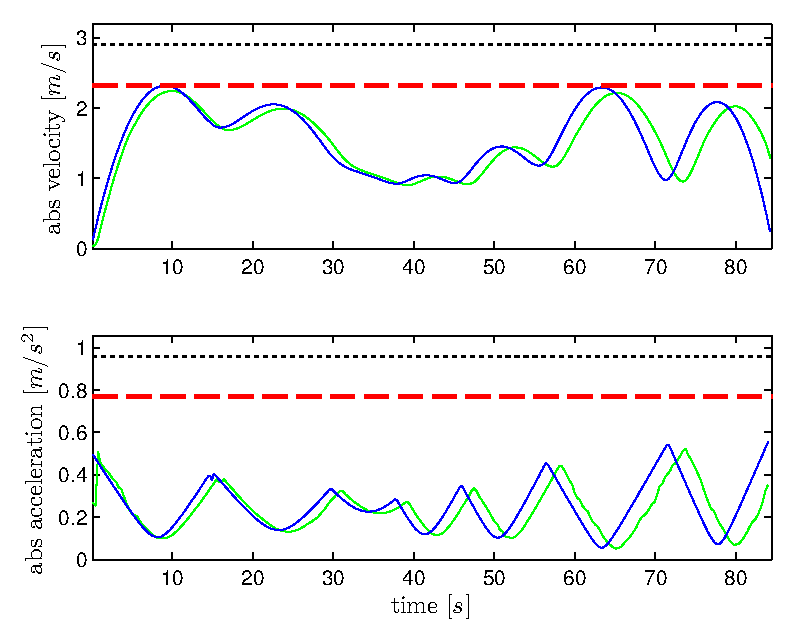
\includegraphics[width = 0.8\textwidth]{sys_constr/figure_1D_agile_SplineDegree3_crossTrack_Disturbance_0_S_125}
  \\ $S=1.25$
  \end{minipage}\\ \hspace{5pt}
  \begin{minipage}[t]{0.48\textwidth}
    \centering
    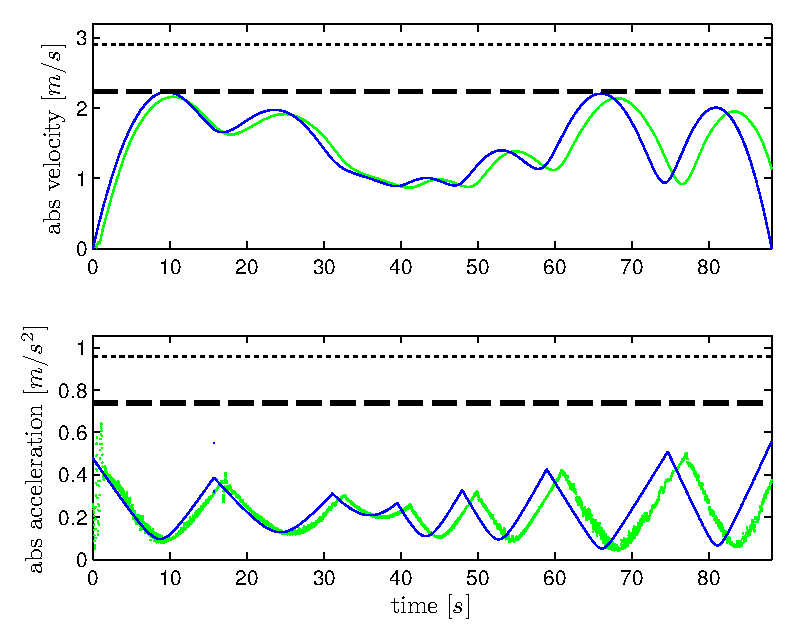
\includegraphics[width = 0.8\textwidth]{sys_constr/figure_1D_agile_SplineDegree3_crossTrack_Disturbance_0_S_130}
  \\ $S=1.3$
  \end{minipage}
  \begin{minipage}[t]{0.48\textwidth}
    \centering
    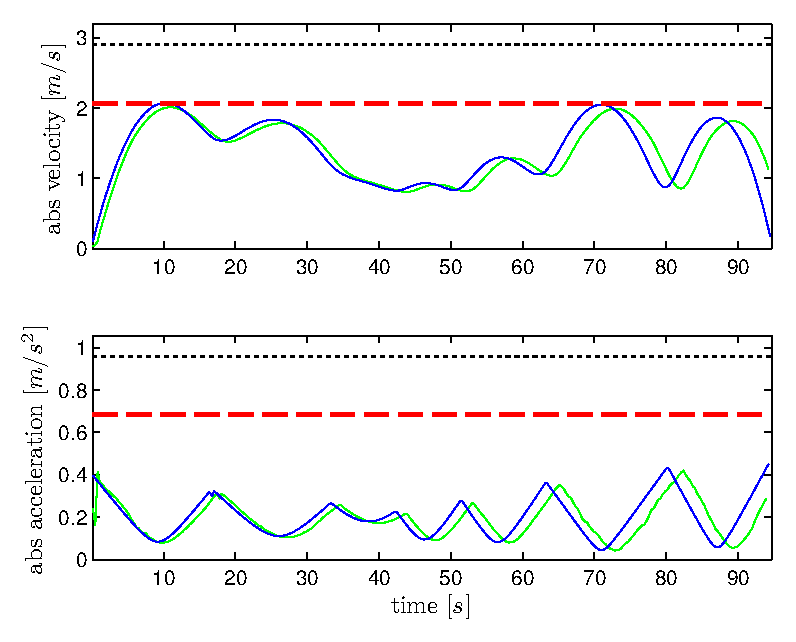
\includegraphics[width = 0.8\textwidth]{sys_constr/figure_1D_agile_SplineDegree3_crossTrack_Disturbance_0_S_140}
  \\ $S=1.4$
  \end{minipage}\\ \hspace{5pt}
  \begin{minipage}[t]{0.48\textwidth}
    \centering
    \includegraphics[width = 0.8\textwidth]{sys_constr/figure_1D_agile_SplineDegree3_crossTrack_Disturbance_0_S_150}
  \\ $S=1.5$
  \end{minipage}
  \begin{minipage}[t]{0.48\textwidth}
    \centering
    \includegraphics[width = 0.8\textwidth]{sys_constr/figure_1D_agile_SplineDegree3_crossTrack_Disturbance_0_S_160}
  \\ $S=1.6$
  \end{minipage} \\
  \label{fig:app_sys_constr}
  \caption{Influence of model accuracy on trajectory controller dynamics. Example using \textit{cross track} controller on \textit{agile} trajectory. For high safety factors ($S=1.6$) the system follows the requested dynamic of the trajectory. For safety factors $S\leq 1$ the maximum dynamics given by the system constraints in \cite{weichart} cannot be reached. Trajectory (blue), trace (green), $(\cdot)_{lim}=(\cdot)_{max}/S$ (dashed bold) and $(\cdot)_{max}$ (dashed)}
\end{figure}



\subsection{Increasing the Path's Curvature}
\label{sub:app_increasing_curvature}
And here follows a subsection with constraint comparisons of a helix with smaller radius.
\\
TO DO
\\
 %\cleardoublepage


%\chapter{Nochmals irgendwas}\label{sec:nochirgendwas}

%Bla bla \dots

 %\cleardoublepage
\section{Mavlink Protocol}
\label{sec:app_mavlink_protocol}

\begin{lstlisting}[captionpos=b, caption="Definition of \textsc{Skye} specific Mavlink messages", label=app_xml]
<?xml version='1.0'?>
<mavlink>
     <include>common.xml</include>
     <enums>
          <enum name="MAV_SKYE_MODE">
               <description>These defines are predefined OR-combined mode flags used for project skye. There is no need to use values from this enum, but it simplifies the use of the mode flags. Note that manual input is enabled in all modes as a safety override.</description>
               <entry value="67" name="MAV_MODE_TESTPHASE_DISARMED">
                    <description>System is ready to test the motors.</description>
               </entry>
               <entry value="195" name="MAV_MODE_TESTPHASE_ARMED">
                    <description>System is ready to test the motors.</description>
               </entry>
               <entry value="65" name="MAV_MODE_DIRECT_CONTROL_DISARMED">
                    <description>System is under Direct Control, no stabilization.</description>
               </entry>
               <entry value="193" name="MAV_MODE_DIRECT_CONTROL_ARMED">
                    <description>System is under Direct Control, no stabilization.</description>
               </entry>
               <entry value="81" name="MAV_MODE_ASSISTED_CONTROL_DISARMED">
                    <description>System is under Assisted Control, stabalized.</description>
               </entry>
               <entry value="209" name="MAV_MODE_ASSISTED_CONTROL_ARMED">
                    <description>System is under Assisted Control, stabalized.</description>
               </entry>
               <entry value="89" name="MAV_MODE_HALF_AUTOMATIC_DISARMED">
                    <description>System is under Half Automatic Control, translation by waypoints, rotation by manual input. Stabalized.</description>
               </entry>
               <entry value="217" name="MAV_MODE_HALF_AUTOMATIC_ARMED">
                    <description>System is under Half Automatic Control, translation by waypoints, rotation by manual input. Stabalized.</description>
               </entry>
               <entry value="93" name="MAV_MODE_FULL_AUTOMATIC_DISARMED">
                    <description>System is under Full Automatic Control, steering by waypoints only. Stabalized.</description>
               </entry>
               <entry value="221" name="MAV_MODE_FULL_AUTOMATIC_ARMED">
                    <description>System is under Full Automatic Control, steering by waypoints only. Stabalized.</description>
               </entry>
          </enum>
          <enum name="MAV_CAM_RECONFIG_PIXEL_CLOCK">
               <description>Camera Reconfigure parameter "color_coding"</description>
               <entry value="6" name="MAV_CAM_RECONFIG_PIXEL_CLOCK_6M">
                    <description/>
               </entry>
               <entry value="8" name="MAV_CAM_RECONFIG_PIXEL_CLOCK_8M">
                    <description/>
               </entry>
               <entry value="10" name="MAV_CAM_RECONFIG_PIXEL_CLOCK_10M">
                    <description/>
               </entry>
               <entry value="13" name="MAV_CAM_RECONFIG_PIXEL_CLOCK_13M5">
                    <description/>
               </entry>
               <entry value="20" name="MAV_CAM_RECONFIG_PIXEL_CLOCK_20M">
                    <description/>
               </entry>
               <entry value="24" name="MAV_CAM_RECONFIG_PIXEL_CLOCK_24M">
                    <description/>
               </entry>
               <entry value="27" name="MAV_CAM_RECONFIG_PIXEL_CLOCK_27M6">
                    <description/>
               </entry>
               <entry value="32" name="MAV_CAM_RECONFIG_PIXEL_CLOCK_32M">
                    <description/>
               </entry>
               <entry value="37" name="MAV_CAM_RECONFIG_PIXEL_CLOCK_37M">
                    <description/>
               </entry>
               <entry value="40" name="MAV_CAM_RECONFIG_PIXEL_CLOCK_40M">
                    <description/>
               </entry>
               <entry value="50" name="MAV_CAM_RECONFIG_PIXEL_CLOCK_50M">
                    <description/>
               </entry>
               <entry value="57" name="MAV_CAM_RECONFIG_PIXEL_CLOCK_57M6">
                    <description/>
               </entry>
          </enum>
          <enum name="MAV_CAM_RECONFIG_COLOR_CODING">
               <description>Camera Reconfigure parameter "color_coding"</description>
               <entry value="0" name="MAV_CAM_RECONFIG_COLOR_CODING_AUTO">
                    <description/>
               </entry>
               <entry value="1" name="MAV_CAM_RECONFIG_COLOR_CODING_MONO8">
                    <description/>
               </entry>
               <entry value="2" name="MAV_CAM_RECONFIG_COLOR_CODING_MONO16">
                    <description/>
               </entry>
               <entry value="3" name="MAV_CAM_RECONFIG_COLOR_CODING_RAW8">
                    <description/>
               </entry>
               <entry value="4" name="MAV_CAM_RECONFIG_COLOR_CODING_BGR8">
                    <description/>
               </entry>
               <entry value="5" name="MAV_CAM_RECONFIG_COLOR_CODING_BGRA8">
                    <description/>
               </entry>
               <entry value="6" name="MAV_CAM_RECONFIG_COLOR_CODING_BGR16">
                    <description/>
               </entry>
          </enum>
          <enum name="MAV_CAM_RECONFIG_BAYER_METHOD">
               <description>Camera Reconfigure parameter "bayer_method"</description>
               <entry value="0" name="MAV_CAM_RECONFIG_BAYER_METHOD_IMAGE_PROC">
                    <description/>Decode via ROS image_proc</entry>
               <entry value="1" name="MAV_CAM_RECONFIG_BAYER_METHOD_DOWNSAMPLE">
                    <description/>DownSample</entry>
               <entry value="2" name="MAV_CAM_RECONFIG_BAYER_METHOD_SIMPLE">
                    <description/>Simple</entry>
               <entry value="3" name="MAV_CAM_RECONFIG_BAYER_METHOD_BILINEAR">
                    <description/>Bilinear</entry>
               <entry value="4" name="MAV_CAM_RECONFIG_BAYER_METHOD_HQ">
                    <description/>HQ</entry>
               <entry value="5" name="MAV_CAM_RECONFIG_BAYER_METHOD_VNG">
                    <description/>VNG</entry>
               <entry value="6" name="MAV_CAM_RECONFIG_BAYER_METHOD_AHD">
                    <description/>AHD</entry>
          </enum>
          <enum name="MAV_CAM_RECONFIG_AUTO_CONTROL_SPEED">
               <description>Camera Reconfigure parameter "auto_control_speed"</description>
               <entry value="0" name="MAV_CAM_RECONFIG_AUTO_CONTROL_SPEED_ACS_MEDIUM">
                    <description>Medium</description>
               </entry>
               <entry value="1" name="MAV_CAM_RECONFIG_AUTO_CONTROL_SPEED_ACS_SLOW">
                    <description>Slow</description>
               </entry>
               <entry value="2" name="MAV_CAM_RECONFIG_AUTO_CONTROL_SPEED_ACS_FAST">
                    <description>Fast</description>
               </entry>
          </enum>
          <enum name="MAV_CAM_RECONFIG_HDR_MODE">
               <description>Camera Reconfigure parameter "hdr_mode"</description>
               <entry value="0" name="MAV_CAM_RECONFIG_AUTO_CONTROL_HDR_MODE_HDR_OFF">
                    <description>Off</description>
               </entry>
               <entry value="1" name="MAV_CAM_RECONFIG_AUTO_CONTROL_HDR_MODE_HDR_FIXED0">
                    <description>Fixed0</description>
               </entry>
               <entry value="2" name="MAV_CAM_RECONFIG_AUTO_CONTROL_HDR_MODE_HDR_FIXED1">
                    <description>Fixed1</description>
               </entry>
               <entry value="3" name="MAV_CAM_RECONFIG_AUTO_CONTROL_HDR_MODE_HDR_FIXED2">
                    <description>Fixed2</description>
               </entry>
               <entry value="4" name="MAV_CAM_RECONFIG_AUTO_CONTROL_HDR_MODE_HDR_FIXED3">
                    <description>Fixed3</description>
               </entry>
               <entry value="5" name="MAV_CAM_RECONFIG_AUTO_CONTROL_HDR_MODE_HDR_FIXED4">
                    <description>Fixed4</description>
               </entry>
               <entry value="6" name="MAV_CAM_RECONFIG_AUTO_CONTROL_HDR_MODE_HDR_FIXED5">
                    <description>Fixed5</description>
               </entry>
               <entry value="7" name="MAV_CAM_RECONFIG_AUTO_CONTROL_HDR_MODE_HDR_FIXED6">
                    <description>Fixed6</description>
               </entry>
               <entry value="8" name="MAV_CAM_RECONFIG_AUTO_CONTROL_HDR_MODE_HDR_USER">
                    <description>User</description>
               </entry>
          </enum>
          <enum name="MAV_CAM_ID">
               <description>Camera ID</description>
               <entry value="0" name="MAV_CAM_ID_ALL">
                    <description>Off</description>
               </entry>
               <entry value="1" name="MAV_CAM_ID_PROSILICA">
                    <description>High resolution AVT prosilica camera</description>
               </entry>
               <entry value="2" name="MAV_CAM_ID_BLUEFOX_LEFT">
                    <description>Low resolution matrix-vision bluefox camera, position left</description>
               </entry>
               <entry value="3" name="MAV_CAM_ID_BLUEFOX_RIGHT">
                    <description>Low resolution matrix-vision bluefox camera, position right</description>
               </entry>
          </enum>
          <enum name="MAV_CAM_IMAGE_FORMAT">
               <description>Image Format</description>
               <entry value="0" name="MAV_CAM_IMAGE_FORMAT_RAW">
                    <description>RAW format</description>
               </entry>
               <entry value="1" name="MAV_CAM_IMAGE_FORMAT_JPEG">
                    <description>JPEG format</description>
               </entry>
               <entry value="2" name="MAV_CAM_IMAGE_FORMAT_PNG">
                    <description>PNG format</description>
               </entry>
	        </enum>
<!-- Copied DATA_TYPES from pixhawk.xml -->
          <enum name="DATA_TYPES">
               <description>Content Types for data transmission handshake</description>
               <entry value="1" name="DATA_TYPE_JPEG_IMAGE"/>
               <entry value="2" name="DATA_TYPE_RAW_IMAGE"/>
               <entry value="3" name="DATA_TYPE_KINECT"/>
          </enum>
          <enum name="MAV_SKYE_BATTERY_PACK_ID">
               <description>ID for each accu pack for detailed battery information</description>
               <entry value="0" name="MAV_SKYE_BATTERY_PACK_ID_NONE">
                    <description>no accu</description>
               </entry>
               <entry value="1" name="MAV_SKYE_BATTERY_PACK_ID_1">
                    <description>Accu pack 1</description>
               </entry>
               <entry value="2" name="MAV_SKYE_BATTERY_PACK_ID_2">
                    <description>Accu pack 1</description>
               </entry>
               <entry value="3" name="MAV_SKYE_BATTERY_PACK_ID_3">
                    <description>Accu pack 1</description>
               </entry>
          </enum>
     </enums>
     <messages>
          <message id="152" name="SKYE_BATTERY_STATUS">
               <description>Transmit battery informations for a accu pack.</description>
               <field type="uint8_t" name="accu_id">Accupack ID, see ENUM MAV_SKYE_BATTERY_PACK_ID</field>
               <field type="uint16_t" name="voltage_cell_1">Battery voltage of cell 1, in millivolts (1 = 1 millivolt)</field>
               <field type="uint16_t" name="voltage_cell_2">Battery voltage of cell 2, in millivolts (1 = 1 millivolt)</field>
               <field type="uint16_t" name="voltage_cell_3">Battery voltage of cell 3, in millivolts (1 = 1 millivolt)</field>
               <field type="uint16_t" name="voltage_cell_4">Battery voltage of cell 4, in millivolts (1 = 1 millivolt)</field>
               <field type="int16_t" name="current_battery">Battery current, in 10*milliamperes (1 = 10 milliampere), -1: autopilot does not measure the current</field>
               <field type="int8_t" name="battery_remaining">Remaining battery energy: (0%: 0, 100%: 100), -1: autopilot estimate the remaining battery</field>
          </message>
          <message id="153" name="SKYE_TEST_MOTORS">
               <description>Message type for project SKYE configuration with four thrusters and four direction actuations. Requested mode: "MAV_MODE_TESTPHASE_ARMED"</description>
               <field type="uint8_t" name="target_system">System ID</field>
               <field type="uint8_t" name="thrust_1">Thrust of motor 1, range [0,200]</field>
               <field type="uint8_t" name="thrust_2">Thrust of motor 2, range [0,200]</field>
               <field type="uint8_t" name="thrust_3">Thrust of motor 3, range [0,200]</field>
               <field type="uint8_t" name="thrust_4">Thrust of motor 4, range [0,200]</field>
               <field type="int16_t" name="direct_1">Direction of direction motor 1, in 0.1 degrees [-360deg: -3600, 360deg: 3600] </field>
               <field type="int16_t" name="direct_2">Direction of direction motor 2, in 0.1 degrees [-360deg: -3600, 360deg: 3600] </field>
               <field type="int16_t" name="direct_3">Direction of direction motor 3, in 0.1 degrees [-360deg: -3600, 360deg: 3600] </field>
               <field type="int16_t" name="direct_4">Direction of direction motor 4, in 0.1 degrees [-360deg: -3600, 360deg: 3600] </field>
          </message>
          <message id="154" name="SKYE_DIRECT_CONTROL">
               <description>Control six degrees of freedom in Body Frame. This type of control is intended to use if there is no attitude feedback in the control. Requested mode: "MAV_MODE_DIRECT_CONTROL_ARMED"</description>
               <field type="uint8_t" name="target_system">System ID</field>
               <field type="float" name="thrust_x">Resulting thrust in Body Frame x, in Newton</field>
               <field type="float" name="thrust_y">Resulting thrust in Body Frame y, in Newton</field>
               <field type="float" name="thrust_z">Resulting thrust in Body Frame z, in Newton</field>
               <field type="float" name="moment_x">Resulting moment in Body Frame x (roll), in Newtonmeter</field>
               <field type="float" name="moment_y">Resulting moment in Body Frame y (pitch), in Newtonmeter</field>
               <field type="float" name="moment_z">Resulting moment in Body Frame z (yaw), in Newtonmeter</field>
          </message>
          <message id="155" name="SKYE_ASSISTED_CONTROL">
               <description>Control six degrees of freedom. Translational velocity in Inertial (earth) Frame. Use this manual control mode with the requested mode: "MAV_MODE_ASSISTED_CONTROL_ARMED"</description>
               <field type="uint8_t" name="target_system">System ID</field>
               <field type="float" name="translation_lat">Translation (velocity) in Inertial Frame latitude, in m/sec</field>
               <field type="float" name="translation_long">Translation (velocity) in Inertial Frame longitude, in m/sec</field>
               <field type="float" name="translation_alt">Translation (velocity) in Inertial Frame altitude, in m/sec</field>
               <field type="float" name="rotation_x">Roll (angular velocity), in rad/sec</field>
               <field type="float" name="rotation_y">Pitch (angular velocity), in rad/sec</field>
               <field type="float" name="rotation_z">Yaw (angular velocity), in rad/sec</field>
          </message>
          <message id="157" name="SKYE_SCALED_PRESSURE">
               <description>The pressure readings for the typical setup of one absolute and differential pressure sensor. The units are as specified in each field. For accurate analysis needed by at least 6Hz.</description>
               <field type="uint32_t" name="time_boot_ms">Timestamp (microseconds since UNIX epoch or microseconds since system boot)</field>
               <field type="float" name="press_abs1">Absolute pressure (hectopascal)</field>
               <field type="float" name="press_diff11">Differential pressure 1 (hectopascal)</field>
               <field type="float" name="press_diff12">Differential pressure 1 (hectopascal)</field>
               <field type="float" name="press_diff13">Differential pressure 1 (hectopascal)</field>
               <field type="float" name="press_abs2">Absolute pressure (hectopascal)</field>
               <field type="float" name="press_diff21">Differential pressure 1 (hectopascal)</field>
               <field type="float" name="press_diff22">Differential pressure 1 (hectopascal)</field>
               <field type="float" name="press_diff23">Differential pressure 1 (hectopascal)</field>
               <field type="float" name="press_abs3">Absolute pressure (hectopascal)</field>
               <field type="float" name="press_diff31">Differential pressure 1 (hectopascal)</field>
               <field type="float" name="press_diff32">Differential pressure 1 (hectopascal)</field>
               <field type="float" name="press_diff33">Differential pressure 1 (hectopascal)</field>
               <field type="float" name="press_abs4">Absolute pressure (hectopascal)</field>
               <field type="float" name="press_diff41">Differential pressure 1 (hectopascal)</field>
               <field type="float" name="press_diff42">Differential pressure 1 (hectopascal)</field>
               <field type="float" name="press_diff43">Differential pressure 1 (hectopascal)</field>
               <field type="int16_t" name="temperature">Temperature measurement (0.01 degrees celsius)</field>
          </message>
          <message id="158" name="SKYE_MOTOR_SIGNAL">
               <description>The values transmitted to the motor nodes.</description>
               <field type="uint32_t" name="time_usec">Timestamp (since UNIX epoch or microseconds since system boot)</field>
               <field type="uint8_t" name="thrust1_raw">Thrust output thruster 1, range [0,200]</field>
               <field type="uint8_t" name="thrust2_raw">Thrust output thruster 2, range [0,200]</field>
               <field type="uint8_t" name="thrust3_raw">Thrust output thruster 3, range [0,200]</field>
               <field type="uint8_t" name="thrust4_raw">Thrust output thruster 4, range [0,200]</field>
               <field type="int16_t" name="position1_raw">Orientation output position motor 1, in 0.1 degrees [-360deg: -3600, 360deg: 3600]</field>
               <field type="int16_t" name="position2_raw">Orientation output position motor 2, in 0.1 degrees [-360deg: -3600, 360deg: 3600]</field>
               <field type="int16_t" name="position3_raw">Orientation output position motor 3, in 0.1 degrees [-360deg: -3600, 360deg: 3600]]</field>
               <field type="int16_t" name="position4_raw">Orientation output position motor 4, in 0.1 degrees [-360deg: -3600, 360deg: 3600]</field>
          </message>
          <message id="159" name="SKYE_MOTOR_MEASSURED_POSITION">
               <description>The meassured orientation of the motors</description>
               <field type="uint32_t" name="time_usec">Timestamp (since UNIX epoch or microseconds since system boot)</field>
               <field type="int16_t" name="pos1_raw">Meassureed orientation motor 1, in 10qc [360deg: 17614]</field>
               <field type="int16_t" name="pos2_raw">Meassureed orientation motor 1, in 10qc [360deg: 17614]</field>
               <field type="int16_t" name="pos3_raw">Meassureed orientation motor 1, in 10qc [360deg: 17614]</field>
               <field type="int16_t" name="pos4_raw">Meassureed orientation motor 1, in 10qc [360deg: 17614]</field>
          </message>
          <message id="160" name="SKYE_CONTROLLER_OUTPUT">
               <description>Output of controller (Input for actuation chain)</description>
               <field type="uint32_t" name="time_usec">Timestamp (since UNIX epoch or microseconds since system boot)</field>
               <field type="float" name="force_x">Signal given from controller to actuation chain, 1 Newton</field>
               <field type="float" name="force_y">Signal given from controller to actuation chain, 1 Newton</field>
               <field type="float" name="force_z">Signal given from controller to actuation chain, 1 Newton</field>
               <field type="float" name="moment_x">Signal given from controller to actuation chain, 1 Newtonmeter</field>
               <field type="float" name="moment_y">Signal given from controller to actuation chain, 1 Newtonmeter</field>
               <field type="float" name="moment_z">Signal given from controller to actuation chain, 1 Newtonmeter</field>
          </message>
          <message id="161" name="SKYE_CAM_RECONFIGURE_BLUEFOX_SETTINGS">
               <description>Message to change all the parameters present in ROS Reconfigure GUI bluefox node</description>
               <field type="uint8_t" name="target_system">System ID</field>
               <!--               <field type="char[32]" name="guid">Serial number of camera, suffix BLUEFOX_ + 8 dec digits (use first camera if null)</field> -->
               <field type="uint8_t" name="cam_id">ID of camera, see ENUM MAV_CAM_ID</field>
               <field type="char[32]" name="frame_id">ROS tf frame of reference, resolved with tf_prefix unless absolute.</field>
               <field type="uint8_t" name="pixel_clock">Pixel clock of image sensor [MHz]. See enum MAV_CAM_RECONFIG_PIXEL_CLOCK</field>
               <field type="float" name="frame_rate">Camera speed (frames per second). Range: 1.0 to 240.0</field>
               <field type="char[32]" name="camera_info_url">Camera calibration URL for this video_mode (uncalibrated if null). </field>
               <field type="uint8_t" name="binning_x">Number of pixels combined for horizontal binning, use device hints if zero. Range: 0 to 4</field>
               <field type="uint8_t" name="binning_y">Number of pixels combined for vertical binning, use device hints if zero. Range: 0 to 4</field>
               <field type="uint16_t" name="roi_width">Width of Region of Interest in unbinned pixels, full width if zero. Range: 0 to 5000</field>
               <field type="uint16_t" name="roi_height">Height of Region of Interest in unbinned pixels, full height if zero. Range: 0 to 5000</field>
               <field type="uint16_t" name="x_offset">Horizontal offset for left side of ROI in unbinned pixels. Range: 0 to 5000</field>
               <field type="uint16_t" name="y_offset">Vertical offset for top of ROI in unbinned pixels. Range: 0 to 5000</field>
               <field type="uint8_t" name="color_coding">Color coding. See enum MAV_CAM_RECONFIG_COLOR_CODING</field>
               <field type="uint8_t" name="bayer_method">Bayer decoding method (default: ROS image_proc). See enum MAV_CAM_RECONFIG_BAYER_METHOD</field>
               <field type="uint8_t" name="exposure">Auto exposure value . Range: 0 to 255</field>
               <field type="uint8_t" name="shutter_auto">boolean. Shutter control state. </field>
               <field type="float" name="shutter_auto_min">Min shutter time [s] in auto mode. Range: 0.0 to 0.1</field>
               <field type="float" name="shutter_auto_max">Max shutter time [s] in auto mode Range: 0.0 to 0.1</field>
               <field type="float" name="shutter">Shutter time [s]. Range: 0.0 to 0.1</field>
               <field type="uint8_t" name="gain_auto">boolean. Gain control state. </field>
               <field type="uint8_t" name="gain_auto_min">Min relative circuit gain [dB] in auto mode. Range: 0.0 to 12.0</field>
               <field type="uint8_t" name="gain_auto_max">Max relative circuit gain [dB] in auto mode. Range: 0.0 to 12.0</field>
               <field type="uint8_t" name="gain">Relative circuit gain [dB]  Range: 0.0 to 12.0</field>
               <field type="uint8_t" name="auto_control_speed">Control speed for automatic features. See enum MAV_CAM_RECONFIG_AUTO_CONTROL_SPEED</field>
               <field type="uint8_t" name="auto_query_values">boolean. Queries settings that are auto controlled. </field>
               <field type="uint8_t" name="hdr_mode">HDR mode. See enum MAV_CAM_RECONFIG_HDR_MODE</field>
               <field type="uint8_t" name="use_ros_time">boolean. Timestamp Image and CameraInfo using ros::Time::now() </field>
          </message>
          <message id="162" name="SKYE_CAM_RECONFIGURE_PROSILICA_SETTINGS">
               <description>Message to change all the parameters present in ROS Reconfigure GUI prosilica node. FIXME: MESSAGE NOT DEFINED YET</description>
               <field type="uint8_t" name="target_system">System ID</field>
               <field type="uint8_t" name="cam_id">ID of camera, see ENUM MAV_CAM_ID (MAV_CAM_ID_PROSILICA)</field>
          </message>
          <message id="163" name="SKYE_CAM_RECONFIGURE_IMAGE_HANDLER">
               <description>Set parameters of image handler which stores images on HDD and steams them via wifi</description>
               <field type="uint8_t" name="target_system">System ID</field>
               <field type="uint8_t" name="cam_id">ID of camera, see ENUM MAV_CAM_ID</field>
               <field type="uint8_t" name="save_image">Boolean, true: image stream is saved as specified in fields below</field>
               <field type="uint8_t" name="save_percent">Percentage of shot images that are stored</field>
               <field type="uint8_t" name="format">Format of saved image, see ENUM MAV_CAM_IMAGE_FORMAT</field>
               <field type="uint8_t" name="png_level">Compression level for png save format (no compr:1, full compr:9)</field>
               <field type="uint8_t" name="jpeg_quality">Compression quality for jpeg save format (lowest quality: 0, highest quality: 100)</field>
               <field type="char[8]" name="frame_name">Frame name, max. 8 characters</field>
               <field type="char[32]" name="path">Path, where images on SKYE should saved to, max. 32 characters</field>
               <field type="uint8_t" name="send_image">Boolean, true: image stream is sent to GS as specified in fields below</field>
               <field type="uint8_t" name="send_percent">Percentage of shot images that are sent</field>
               <field type="uint8_t" name="format2">Format of sent image, see ENUM MAV_CAM_IMAGE_FORMAT</field>
               <field type="uint8_t" name="png_level2">Compression level for png send format (no compr:1, full compr:9)</field>
               <field type="uint8_t" name="jpeg_quality2">Compression quality for jpeg send format (lowest quality: 0, highest quality: 100)</field>
               <field type="uint8_t" name="keep_old_modus">Boolean, true: new image handle modus is added to previous (image is saved/sent more than once), false: only 
save/send with new configuration</field>
          </message>
          <message id="164" name="SKYE_CAM_TAKE_SHOT">
               <description>Take a single shot and store the image via ROS on groundstation</description>
               <field type="uint8_t" name="target_system">System ID</field>
               <field type="uint8_t" name="cam_id">ID of camera, see ENUM MAV_CAM_ID</field>
               <field type="uint8_t" name="take_shot">Boolean, true: send recent image (save settings) to GS</field>
          </message>
          <message id="165" name="SKYE_CAM_IMAGE_TRIGGERED">
               <description>This message indicates that there is a new image in default local path that can be displayed in QGC. Use this message only if you do NOT transmit the image via the mavlink protocol (ENCAPSULED_DATA)</description>
               <field type="uint64_t" name="timestamp">Timestamp</field>
               <field type="uint8_t" name="cam_id">ID of camera, see ENUM MAV_CAM_ID</field>
               <!--               <field type="uint32_t" name="seq">IMU seq</field>      -->
               <field type="float" name="roll">Roll angle in rad</field>
               <field type="float" name="pitch">Pitch angle in rad</field>
               <field type="float" name="yaw">Yaw angle in rad</field>
               <!--               <field type="float" name="local_z">Local frame Z coordinate (height over ground)</field>   -->
               <field type="int32_t" name="lat">Latitude, expressed as * 1E7</field>
               <field type="int32_t" name="lon">Longitude, expressed as * 1E7</field>
               <field type="int32_t" name="alt">Altitude in meters, expressed as * 1000 (millimeters), above MSL</field>
               <!--               <field type="float" name="ground_x">Ground truth X</field>			
               <field type="float" name="ground_y">Ground truth Y</field>
               <field type="float" name="ground_z">Ground truth Z</field>		-->
          </message>
          <message id="166" name="SKYE_HOME_MAXON">
              <description/>
              <field type="uint8_t" name="target_system">System ID</field>
              <field type="uint8_t" name="homing">Boolean, true: home maxon motors</field>
         </message>
         <message id="167" name="SKYE_THREAD_COUNTS">
               <description>Info about running threads on autopilot</description>
               <field type="uint32_t" name="time_usec">Timestamp (since UNIX epoch or microseconds since system boot)</field>
               <field type="uint8_t" name="running_threads">Number of running threads</field>
               <field type="uint64_t" name="heartbeatloop_count">Counter of heartbeatloop</field>
               <field type="uint64_t" name="receiveloop_count">Counter of receiveloop</field>
               <field type="uint64_t" name="telemetryloop_count">Counter of telemetryloop</field>
               <field type="uint64_t" name="gyroaccloop_count">Counter of gyroaccloop</field>
               <field type="uint64_t" name="controlloop_count">Counter of controlloop</field>
               <field type="uint64_t" name="stateestimation_count">Counter of stateestimation</field>
          </message>
         <message id="168" name="SKYE_THREAD_USLEEP">
               <description>Info about running threads on autopilot</description>
               <field type="uint32_t" name="time_usec">Timestamp (since UNIX epoch or microseconds since system boot)</field>
               <field type="int64_t" name="heartbeatloop_usleep">Microseconds heartbeatloop is sleeping</field>
               <field type="int64_t" name="receiveloop_timestamp">Microseconds receiveloop is sleeping</field>
               <field type="int64_t" name="telemetryloop_usleep">Microseconds telemetryloop is sleeping</field>
               <field type="int64_t" name="gyroaccloop_usleep">Microseconds gyroaccloop is sleeping</field>
               <field type="int64_t" name="controlloop_usleep">Microseconds controlloop is sleeping</field>
               <field type="int64_t" name="stateestimation_usleep">Microseconds stateestimation loop is sleeping</field>
          </message>
          <message id="169" name="SKYE_REQUEST_CAM_RECONFIGURE_SETTINGS">
               <description>Request to transmit the current camera reconfigure settings of camera specified by cam_id</description>
               <field type="uint8_t" name="target_system">System ID</field>
               <field type="uint8_t" name="cam_id">ID of camera, see ENUM MAV_CAM_ID</field>
          </message>
          <message id="170" name="SKYE_REQUEST_CAM_RECONFIGURE_HANDLER">
               <description>Request to transmit the current image handler settings of camera specified by cam_id</description>
               <field type="uint8_t" name="target_system">System ID</field>
               <field type="uint8_t" name="cam_id">ID of camera, see ENUM MAV_CAM_ID</field>
          </message>
<!-- DATA_TRANSMISSION_HANDSHAKE and ENCAPSULATED_DATA copied from pixhawk.xml -->
          <message id="193" name="DATA_TRANSMISSION_HANDSHAKE">
               <description>Tell QGC that a new image will be transmitted as ENCAPSULATED_DATA</description>
               <field type="uint8_t" name="type">type of requested/acknowledged data (as defined in ENUM DATA_TYPES in mavlink/include/mavlink_types.h)</field>
               <field type="uint32_t" name="size">total data size in bytes (set on ACK only)</field>
               <field type="uint16_t" name="width">Width of a matrix or image</field>
               <field type="uint16_t" name="height">Height of a matrix or image</field>
               <field type="uint8_t" name="packets">number of packets beeing sent (set on ACK only) </field>
               <field type="uint8_t" name="payload">payload size per packet (normally 253 byte, see DATA field size in message ENCAPSULATED_DATA) (set on ACK only) </field>
               <field type="uint8_t" name="jpg_quality">JPEG quality out of [1,100]</field>
          </message>
          <message id="194" name="ENCAPSULATED_DATA">
               <description>Split image into mavlink packages to send it in the data array</description>
               <field type="uint16_t" name="seqnr">sequence number (starting with 0 on every transmission)</field>
               <field type="uint8_t[253]" name="data">image data bytes</field>
          </message>
     </messages>
</mavlink>
\end{lstlisting}